%% ----------------------------------------------------------------
%% Thesis.tex -- MAIN FILE (the one that you compile with LaTeX)
%% ----------------------------------------------------------------

% Set up the document
\documentclass[a4paper, 11pt, oneside]{Thesis}  % Use the "Thesis" style, based on the ECS Thesis style by Steve Gunn
\graphicspath{Figures/}  % Location of the graphics files (set up for graphics to be in PDF format)

% Include any extra LaTeX packages required
\usepackage[square, numbers, comma, sort&compress]{natbib}  % Use the "Natbib" style for the references in the Bibliography
\usepackage{verbatim}  % Needed for the "comment" environment to make LaTeX comments
\usepackage{vector}  % Allows "\bvec{}" and "\buvec{}" for "blackboard" style bold vectors in maths
\hypersetup{urlcolor=blue, colorlinks=true}  % Colours hyperlinks in blue, but this can be distracting if there are many links.

%% ----------------------------------------------------------------
\begin{document}
\frontmatter      % Begin Roman style (i, ii, iii, iv...) page numbering

% Set up the Title Page
\title  {An evaluation of touch-based music sequencer apps on iPad}
\authors  {\texorpdfstring
            {{Ke Ding}}
            {Ke Ding}
            }
\addresses  {\groupname\\\deptname\\\univname}  % Do not change this here, instead these must be set in the "Thesis.cls" file, please look through it instead
\date       {\today}
\subject    {}
\keywords   {}

\maketitle
%% ----------------------------------------------------------------

\setstretch{1.3}  % It is better to have smaller font and larger line spacing than the other way round

% Define the page headers using the FancyHdr package and set up for one-sided printing
\fancyhead{}  % Clears all page headers and footers
\rhead{\thepage}  % Sets the right side header to show the page number
\lhead{}  % Clears the left side page header

\pagestyle{fancy}  % Finally, use the "fancy" page style to implement the FancyHdr headers

%% ----------------------------------------------------------------
% Declaration Page required for the Thesis, your institution may give you a different text to place here
\Declaration{

\addtocontents{toc}{\vspace{1em}}  % Add a gap in the Contents, for aesthetics

I, AUTHOR NAME, declare that this thesis titled, `THESIS TITLE' and the work presented in it are my own. I confirm that:

\begin{itemize}
\item[\tiny{$\blacksquare$}] This work was done wholly or mainly while in candidature for a research degree at this University.

\item[\tiny{$\blacksquare$}] Where any part of this thesis has previously been submitted for a degree or any other qualification at this University or any other institution, this has been clearly stated.

\item[\tiny{$\blacksquare$}] Where I have consulted the published work of others, this is always clearly attributed.

\item[\tiny{$\blacksquare$}] Where I have quoted from the work of others, the source is always given. With the exception of such quotations, this thesis is entirely my own work.

\item[\tiny{$\blacksquare$}] I have acknowledged all main sources of help.

\item[\tiny{$\blacksquare$}] Where the thesis is based on work done by myself jointly with others, I have made clear exactly what was done by others and what I have contributed myself.
\\
\end{itemize}


Signed:\\
\rule[1em]{25em}{0.5pt}  % This prints a line for the signature

Date:\\
\rule[1em]{25em}{0.5pt}  % This prints a line to write the date
}
\clearpage  % Declaration ended, now start a new page

%% ----------------------------------------------------------------
% The "Funny Quote Page"
\pagestyle{empty}  % No headers or footers for the following pages

\null\vfill
% Now comes the "Funny Quote", written in italics
\textit{``Write a funny quote here.''}

\begin{flushright}
If the quote is taken from someone, their name goes here
\end{flushright}

\vfill\vfill\vfill\vfill\vfill\vfill\null
\clearpage  % Funny Quote page ended, start a new page
%% ----------------------------------------------------------------

% The Abstract Page
\addtotoc{Abstract}  % Add the "Abstract" page entry to the Contents
\abstract{
\addtocontents{toc}{\vspace{1em}}  % Add a gap in the Contents, for aesthetics

The Thesis Abstract is written here (and usually kept to just this page). The page is kept centered vertically so can expand into the blank space above the title too\ldots

}

\clearpage  % Abstract ended, start a new page
%% ----------------------------------------------------------------

\setstretch{1.3}  % Reset the line-spacing to 1.3 for body text (if it has changed)

% The Acknowledgements page, for thanking everyone
\acknowledgements{
\addtocontents{toc}{\vspace{1em}}  % Add a gap in the Contents, for aesthetics

The acknowledgements and the people to thank go here, don't forget to include your project advisor\ldots

}
\clearpage  % End of the Acknowledgements
%% ----------------------------------------------------------------

\pagestyle{fancy}  %The page style headers have been "empty" all this time, now use the "fancy" headers as defined before to bring them back


%% ----------------------------------------------------------------
\lhead{\emph{Contents}}  % Set the left side page header to "Contents"
\tableofcontents  % Write out the Table of Contents

%% ----------------------------------------------------------------
\lhead{\emph{List of Figures}}  % Set the left side page header to "List if Figures"
\listoffigures  % Write out the List of Figures

%% ----------------------------------------------------------------
\lhead{\emph{List of Tables}}  % Set the left side page header to "List of Tables"
\listoftables  % Write out the List of Tables

%% ----------------------------------------------------------------
\setstretch{1.5}  % Set the line spacing to 1.5, this makes the following tables easier to read
\clearpage  % Start a new page
\lhead{\emph{Abbreviations}}  % Set the left side page header to "Abbreviations"
\listofsymbols{ll}  % Include a list of Abbreviations (a table of two columns)
{
% \textbf{Acronym} & \textbf{W}hat (it) \textbf{S}tands \textbf{F}or \\
\textbf{LAH} & \textbf{L}ist \textbf{A}bbreviations \textbf{H}ere \\

}

%% ----------------------------------------------------------------
\clearpage  % Start a new page
\lhead{\emph{Physical Constants}}  % Set the left side page header to "Physical Constants"
\listofconstants{lrcl}  % Include a list of Physical Constants (a four column table)
{
% Constant Name & Symbol & = & Constant Value (with units) \\
Speed of Light & $c$ & $=$ & $2.997\ 924\ 58\times10^{8}\ \mbox{ms}^{-\mbox{s}}$ (exact)\\

}

%% ----------------------------------------------------------------
\clearpage  %Start a new page
\lhead{\emph{Symbols}}  % Set the left side page header to "Symbols"
\listofnomenclature{lll}  % Include a list of Symbols (a three column table)
{
% symbol & name & unit \\
$a$ & distance & m \\
$P$ & power & W (Js$^{-1}$) \\
& & \\ % Gap to separate the Roman symbols from the Greek
$\omega$ & angular frequency & rads$^{-1}$ \\
}
%% ----------------------------------------------------------------
% End of the pre-able, contents and lists of things
% Begin the Dedication page

\setstretch{1.3}  % Return the line spacing back to 1.3

\pagestyle{empty}  % Page style needs to be empty for this page
\dedicatory{For/Dedicated to/To my\ldots}

\addtocontents{toc}{\vspace{2em}}  % Add a gap in the Contents, for aesthetics


%% ----------------------------------------------------------------
\mainmatter	  % Begin normal, numeric (1,2,3...) page numbering
\pagestyle{fancy}  % Return the page headers back to the "fancy" style

% Include the chapters of the thesis, as separate files
% Just uncomment the lines as you write the chapters

\pagestyle{fancy}
\rhead{\thepage}
\lhead{Introduction}
\chapter{Introduction}

With the rapid development of digital audio technolodge, people start to find out that computers are playing an increasingly important role in music. This new trend is providing unprecedented opportunities for people to create and manipulate sound. However, the flexibility of the digital technolodge is accompanied by confuse and uncertainty. As a result, thousands of new musicial forms built on computers have been created and released to the world. And it is natural to ask, what kinds of musical interfaces are taking better advantage of computers. To answer this question, researchers targeting at the better establised field of human-computer interaction \citep{Reference16}. Under the circumstance of new musical form explosion, a new community called NIME was born (see \ref{subsec: nime}).

\section{Background}
\label{sec: backgound}

\subsection{The development of NIME}
\label{subsec: nime}
% what is NIME and it's development
The New Interface for Musical Expression (NIME) is an international conference for musicians and researchers from all over the world to demonstrate their latest work on musical interface design \citep{Reference15}. It first started as a workshop at the Conference on Human Factors in Computing System (CHI) in 2001. After that, annually conferences have been held around the world. The hoster are research groups who devote themselves to interface design, human-computer interaction and computer music. The latest conference was held at Griffith University in Brisbane, Queensland, Australia in 2016.

In the last sixteen years, NIME has explored different approaches on new musical interface design. The \textit{reacTable} which was designed for live music performance on tabletop led a new trend on tangible music interface \citep{Reference17}. Many researchers shifted their attention to this new media. Toolkit such as reacTiVision was developed to detect movement of performers and allow further development to turn any surface into a musical instrument \citep{Reference18}.

The success of \textit{Smule} initiated a new era of mobile music \citep{Reference8}. After that, thousands of musical applications such as \textit{MoMu, MadPad and Magic Fiddle} which were specifically designed for mobile devices were developed \citep{Reference8.2,Reference8.3,Reference8.4}.



\subsection{iPad: a new playground for musicians}
% we will first brefly introduce the ipad, and then illustrate the strength of ipad. also the reason why we major investigate on ipad

The iPad, a tablet computer with touchscreen display, has quickly occupied the market all around world since it's first release in 2010 \citep{Reference2}. The emergence of iPad have provided a new platform for users to explore digital world \citep{Reference1}. After 7 generations, the usage of iPad has shifted from the extension of iPhone to a powerful pruductivity tool. In this shift, thousands of applications which was designed to utilise the larger touch screen has emerged. According to Daniel, there are over 1.5 million apps are currently hosted in the App Store and more than half of those apps are specifically designed for iPad \citep{lifewire}.

Since the first release of iPad, there are practices to utilise the large tangible screen and wide variety of sensors of this cross-time product. \citeauthor{Reference8.4} designed \textit{Magic Fiddle}, a new musical instrument, which combined the physical gesture of users and graphical display of iPad together. \citeauthor{Reference19} explored the possibility of using iPad as a percussive instrument and used iPad's network feature to ecourage cohesive improvisation \citep{Reference19}.

\section{Related Work}

A lot of work have been down on evluating the interaction between users and mobile devices such as iPhone. However, there haven't been a paper specificly analyze musical instrument implemented on iPad. \citeauthor{Reference21} evaluated the live music-making on computer through discourse analysis and turing test \citep{Reference21}. A questionnaire-based evaluation method was proposed to evaluate the musical instruments, especially the new forms of instruments from NIME \citep{Reference0}.

Unexpectedly, music sequencers as the top three most popular instruments in iOS musical applications \citep{Reference14}, has not attracted much attention. We can barely find papers related to recent years development of music sequencers application. The most related work was \textit{Block Jam} (see figure \ref{fig: Block Jam}), a sequencer with tangible interface consisited of several physical blocks \citep{Reference20}.

\bigskip
\begin{figure}[h]
  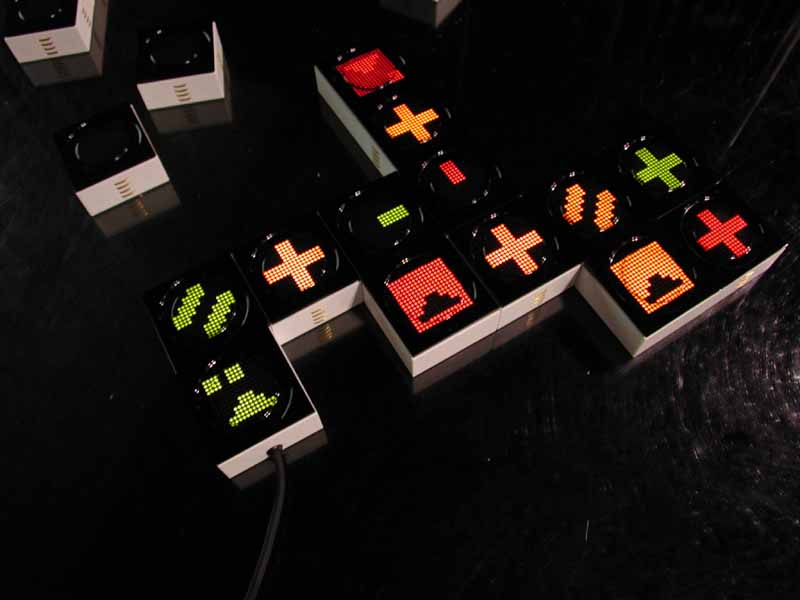
\includegraphics[width=12 cm]{images/blockjam.jpg}
  \centering
  \caption{Block Jam: music sequencer consist of a cluster of blocks}
  \label{fig: Block Jam}
\end{figure}
\bigskip

\section{Research goals and motivation}

While musical interfaces have been studied for a long time, there have emerged thousands of novel twists on \textquotedblleft{grid-based}\textquotedblright music sequencer. And to our knowledge there is currently no paper investigate the situation of this certain kind of musical application on App Store. What's more, there is no consensus on using what's method to evaluate those newborn musical application on mobile devices. This work is a first attempt to classify the music sequencers on iPad and adopt the evaluation method(MPX-Q Questionnaire) designed for NIME community. This work is guided by the following goals:
\begin{flushleft}
$\bullet$ Create an interface taxonomy of current music sequencer apps on the iOS app store.\\
$\bullet$ Perform a HCI user study to measure user experience and musicians performance with different interface design approaches.\\
$\bullet$ Propose design guidlines for musicians, developers and researcher for creating musical interface in the future.
\end{flushleft}
\section{Structure}

In the next chapter, literature relevant to the research topic was introduced, so as to establish a theoretical framework of the research (see Chapter \ref{ch: chapter 2}). And the research project was divided into two consecutive studies. In the first study, we analyzed the music sequencer applications (designed for iPad) on App Store and create an interface taxonomy (see Chapter \ref{ch: chapter 3}). Then base on the classification of music sequencer interfaces, we selected one most representative application from each category and conducted an user study to evlauate the effect of different interface design (see Chapter \ref{ch: chapter 4}). In Chapter \ref{ch: chapter 5}, we discussed the results and provided a conclusion of the study as well as the future work.
 % Introduction

%\pagestyle{fancy}
\rhead{\thepage}
\lhead{Literature Review}
\chapter{Literature Review}
\label{ch: chapter 2}

\section{The development of NIME}
\label{subsec: nime}
% what is NIME and it's development
The New Interfaces for Musical Expression (NIME) conference is an international conference for musicians and researchers from all over the world to demonstrate their latest work on musical interface design \citep{Reference15}. It first started as a workshop at the Conference on Human Factors in Computing System (CHI) in 2001. After that, annually conferences have been held around the world. The hoster are research groups who devote themselves to interface design, human-computer interaction and computer music. The latest conference was held at Griffith University in Brisbane, Queensland, Australia in 2016.

In the last sixteen years, NIME has explored different approaches on new musical interface design. The \textit{reacTable} which was designed for live music performance on tabletop led a new trend on tangible music interface \citep{Reference17}. Many researchers shifted their attention to this new media. Toolkit such as reacTiVision was developed to detect movement of performers and allow further development to turn any surface into a musical instrument \citep{Reference18}.

The success of \textit{Smule} initiated a new era of mobile music \citep{Reference8}. After that, thousands of musical applications such as \textit{MoMu, MadPad and Magic Fiddle} which were specifically designed for mobile devices were developed \citep{Reference8.2,Reference8.3,Reference8.4}.


\section{Mobile Music}

With the increasing popularity of mobile device such as smart phone and tablet, a new research field called Mobile Music emerged \citep{Reference4}. According to the definition by \citeauthor{Reference6}, \textit{Mobile Music} wich employing portable technolodge does not only include the scope of playing music, but also involve music composing, synthesizing and sharing\citep{Reference6}.

In the last sixteen years, there is a growing number of researchers start concerning the development of applications in mobile devices. This new trend was first highlighted by \citeauthor{Reference12} after analysing 98 NIME procedding papers related to mobile music during the period from 2002 to 2012\citep{Reference12}.

The expanding capabilities of mobile devices inspired researchers to exploit the new features.The wireless network ability of mobile device is the first area attract researchers' attention. TunA is the first practice of building connection among PDA users though wireless network\citep{Reference7}. By accessing the playlists of nearby users, TunA help users in same network to exchange their music. \citeauthor{Reference5} extended \citeauthor{Reference7}'s work from music sharing towards collaborative musical creation \citep{Reference5}. \citeauthor{Reference5} propsed a system which exploits ad-hoc wireless networks to allow a community of people using their PDA to work on the same piece of music \citep{Reference5}. Some research started from a different approach by investigating the possibility of utilizing the touch screen on the mobile devices. Geiger designed a paradigm for using touch screen on mobile device like iPaq \citep{Reference9, Reference10}.
MoGMI, which stand for Mobile Gesture Music Instrument, is a research project focused on using the accelorometer inside the mobile phone to perform music. Through examing three different axis mapping models, \citeauthor{Reference11} explored how to turn mobile phone into a standard instrument. Smule Ocarina is the most successful mobile musical artifact, which take advantanges of the global popularity of iPhone \citep{Reference8.1}. It leveraged the microphone to take input from breath, and combined with command from the multitouch screen to mimic the physical interaction of ocarina. Besides, Smule Ocarina also utilizing the GPS module to connect users all around the world and create a new social experience \citep{Reference8}.


\section{Musical Interaction Patterns and Sequencer}
% in this section we are going to introduce several major interaction patternn in mobile devices bath on \cite{Reference4}
Musical interaction patterns, also konw as design patterns, are common solutions for developers to design a specific interface,like music sequencer. \citeauthor{Reference4} stated since designer can reuse the proven discipline in their work, design patterns can assisit multidisciplinary design, improve communication between designers and facilaitae knowledage transfer between teams with different background \citep{Reference4}. In \citeauthor{Reference4}'s work, following four most common music interaction patters on mobile devices were given:
1). Natural Interaction. 2). Event Sequencing. 3). Process Control 4). Sound Mixing.
In which, event sequencing was the second most popular interaction patterns. The general decription of event sequencing pattern was illustrated as: editing the sequence of musical event which maybe individual notes, several piece of samples or parameters that can modify the sound of music \citep{Reference4}. In \citeauthor{Reference13}'s paper, sequencer was put into an independent category of musical application on App Store, and it's nature of mapping was briefly discussed.


\section{Evaluation of digital musical instruments}

Digital musical instruments (DMIs) refer to instruments whose sound are generated digitally. It is not uncommon to ask what does evaluation means in the context of digital musical instruments. But as \citeauthor{Reference25} mentioned, evluating the expressivness and creativity of an musical interface were very difficult \citep{Reference25}. \citeauthor{Reference25}'s paper followed by providing a methodology based on discourse analysis. An evaluation framework was given by \citeauthor{Reference22}, in which DMIs were evaluated from four interdependent prosepective: audience, performer, designer and manufacturer \citep{Reference22}. Also, three general design goals were listed at \citeauthor{Reference22}'s paper, which were \textit{Enjoyment, Playability and Robustness}. \citeauthor{Reference23} proposed a process to evaluate DMIs from a performer's view \citep{Reference23}. A case study conducted by \citeauthor{Reference24} was focued on the expressiveness and mapping of DMIs. Recently, by reviewed 89 papers published in NIME from 2012 to 2014, \citeauthor{Reference26} pushed forward the discussion to how to better use the evaluation tools to improve the design of DMIs \citep{Reference26}. \citeauthor{Reference0} proposed a questionnaire to evaluate the experiential qualities of musical instruments in NIME \citep{Reference0}. \citeauthor{Reference0} indicated the following criteria for musicians to perceive musical instruments:
\begin{flushleft}
  \qquad \qquad $\bullet$ \textbf{Experienced freedom and possibilities (EFP)}\\
  \qquad \qquad $\bullet$ \textbf{Perceived control and comfort (PCC)} \\
  \qquad \qquad $\bullet$ \textbf{Perceived stability, sound quality and aesthetics (PSSQA)}\\
\end{flushleft}
\textit{EFP} as the predominent facet, mainly targets at evaluating the musicianship and expressivity of music instruments. For example, questions like\textit{\textquotedblleft{The instrument allows me to express myself.}\textquotedblright} are used to decide whether the instruments can let muscians to express themselves; \textit{PCC} is used to assess the controbility of the music instruments. Questions such as \textit{\textquotedblleft{I can control the sound appropriately.}\textquotedblright} are setted to identify how well the musicians believed they can control the instruments; \textit{PSSQA} is the most unique facet which analyses the quality of the instruments from the material, the sound and the apperience perspectives. For instance, questions like\textit{\textquotedblleft The instrument pleases me sound-wise\textquotedblright} test the sound quality of the instrument. The above three interrelated facets construct the framework of MPX-Q questionnaire.

\clearpage
 % Background Theory

%\chapter{Study 1: Classification of music sequencer}
\label{ch: chapter 3}

A big scale study was conducted to create an interface taxonomy of current music sequencer apps on the iOS App Store. In total, 55 music sequencer applications on App Store have been examined (see Appendix \ref{app:Appendix A}). Several search criteria are implemented to locate music sequencer on the App Store (see Section\ref{subsec: search criteria}). After analyzing those music sequencer apps, we proposed classification criteria based on the design of the user interface (see Section \ref{sec: classify criteria}). The 55 music sequencer applications were classify into 3 major groups according to the classification criteria (see Section\ref{sec: result}).

\section{Method}
\label{sec:method}

In total, 71 musical iOS applications associated with music sequencer had been downloaded from App Store. After examined and discussed with my supervisor Ben Swift, 16 applications were removed from the study list either because the application can hardly be classified as music sequencer or because the application was not designed for iPad. The rest 55 music sequencer applications were studied in detailed.

\subsection{Search Criteria}
\label{subsec: search criteria}

Base on \citeauthor{Reference13}'s study which created a whitelisted words for music sequencer, keywords such asrt \textit{Sequence, Sequencer, Groovebox, Beatbox, Step, MIDI, Pattern, Tempo, BPM, Machine} were used to search on the App Store. Before each application been downloaded, it's description had been briefly overviewed to make sure it was designed for music purpose. Also, in the searching criteria, \textquotedblleft{iPad only}\textquotedblright was chose and results were sorted under the relevance of keywords.

\subsection{Classification criteria}
\label{sec: classify criteria}
The different approaches of interacting with the applications were used to classify the user interface of the music sequencer applications into several categories. The mappings of the sequencer were broke down into 4 operations,
which were \textit{changing pitch, triggering sound, timing and changing timber}.

\textbf{Changing Pitch.} Becasue the way most traditional instruments' pitch were changed discretely, for example, piano, guitar and violin. The majority of musical application including sequencer follow this trend. Besides, pitch is dominated by grid-like, buttom-to-top mapping in music sequencer hardware. Therefore, grid-based, buttome-to-top and discrete pitches layout is widely adopted.

\bigskip
\begin{figure}[h]
  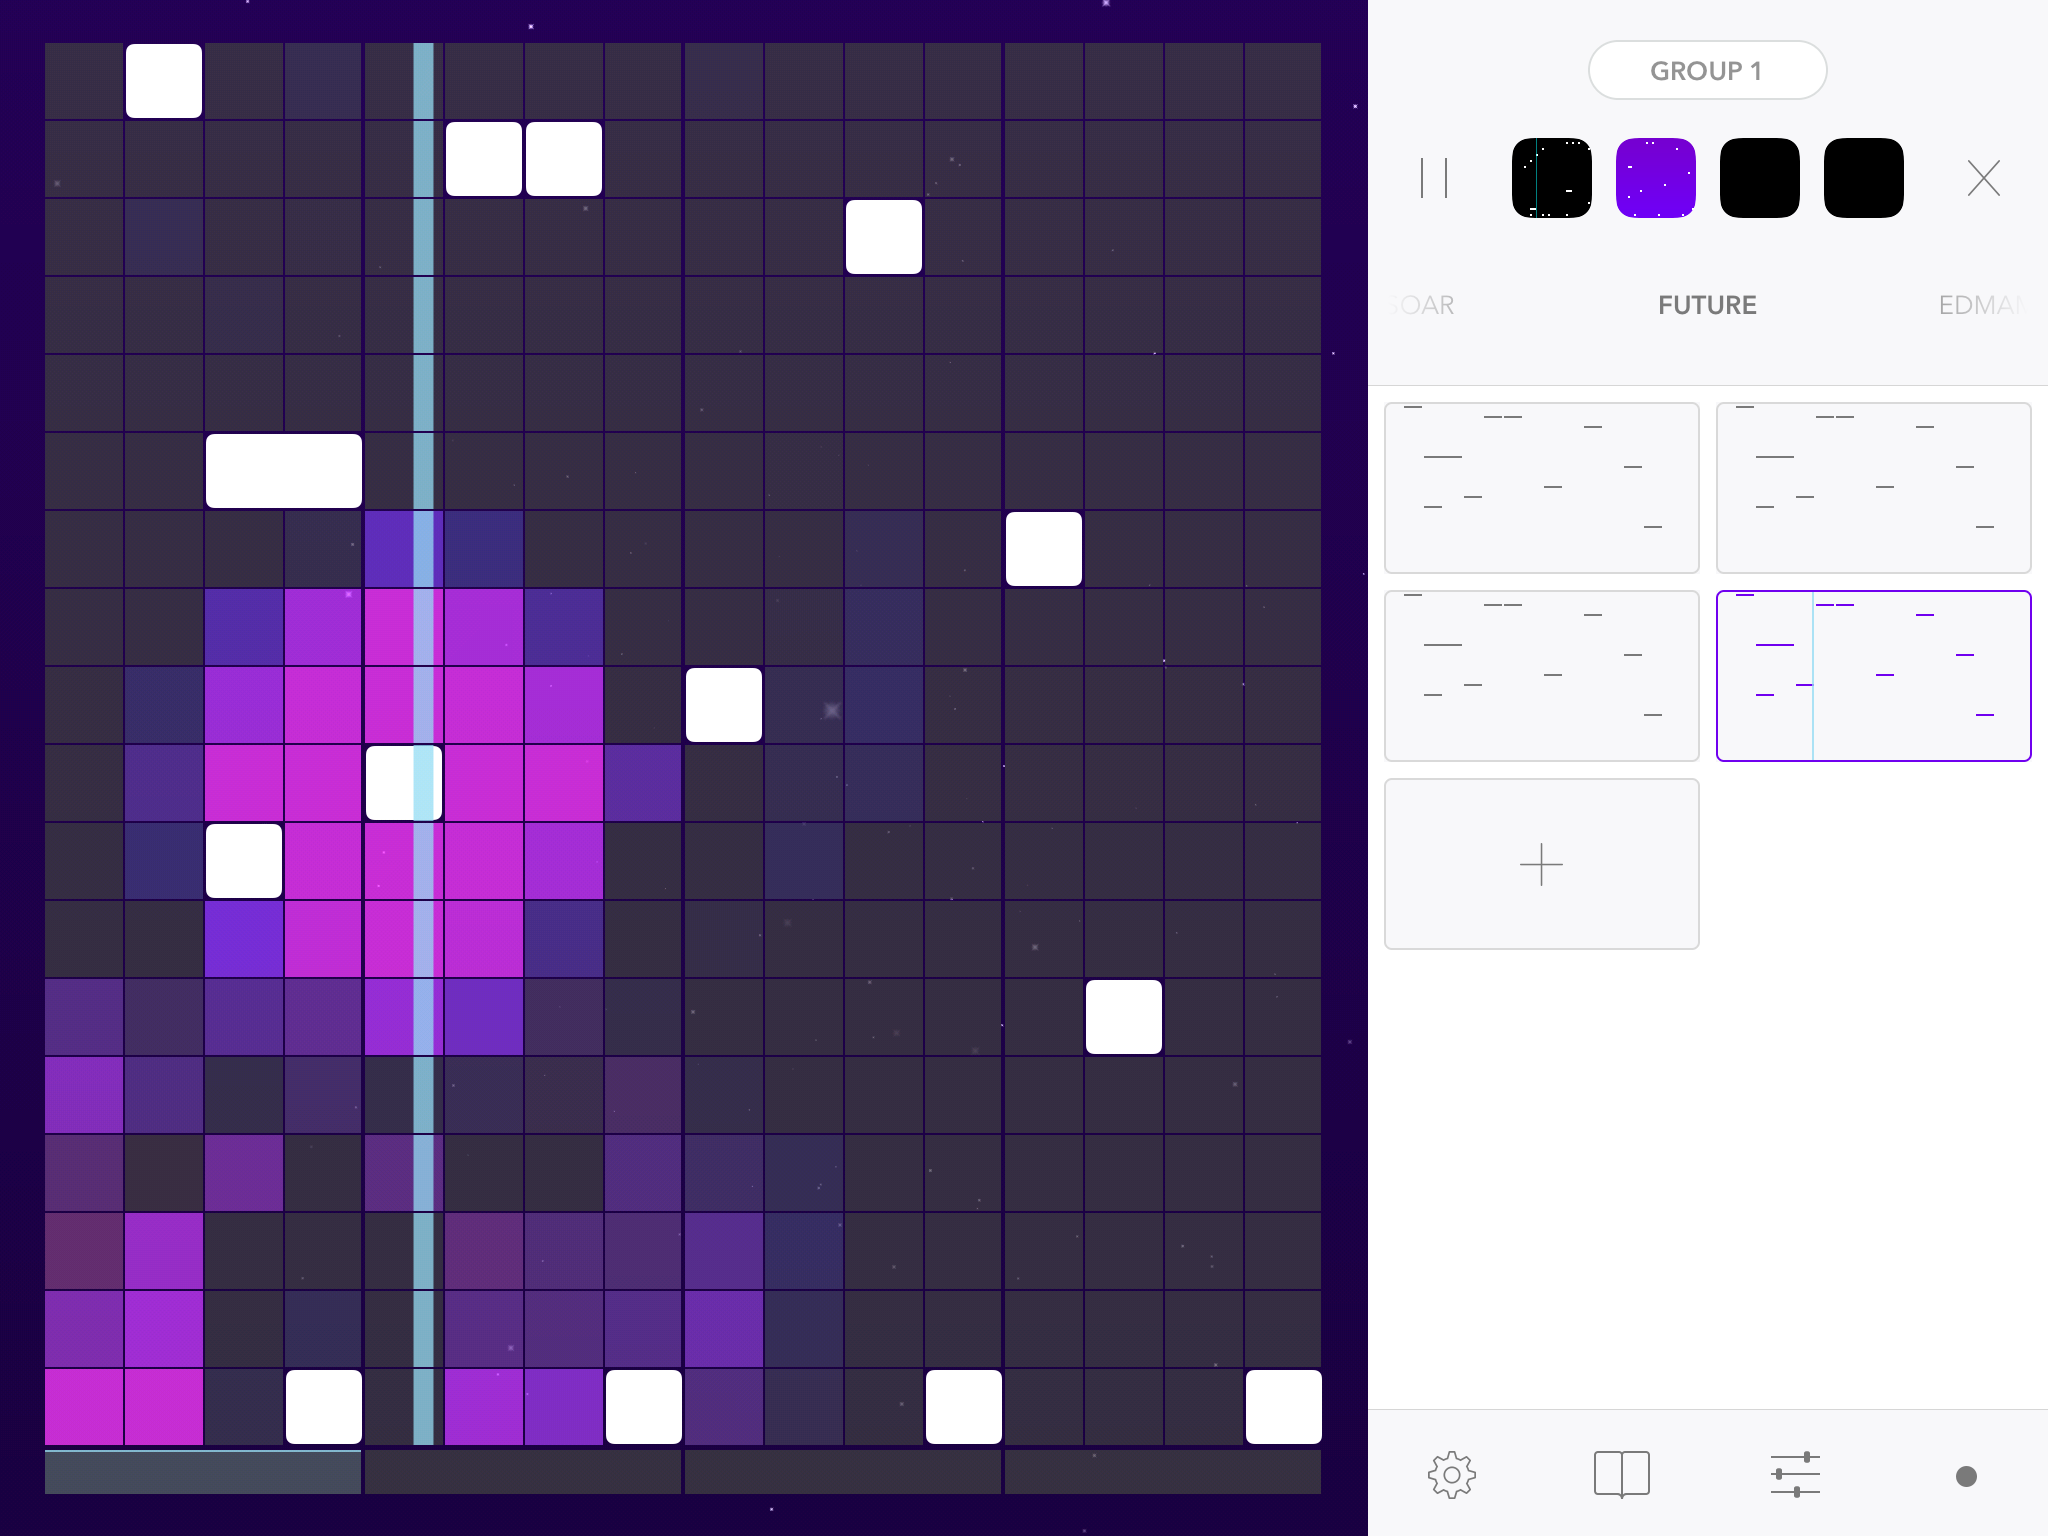
\includegraphics[width=12 cm]{images/Beatwave.PNG}
  \centering
  \caption{Beatwave: grid-based, buttome-to-top and discrete pitch layout}
  \label{fig: Beatwave}
\end{figure}
\bigskip

 Figure \ref{fig: Beatwave} is a good example of this classic interface, in which the interface is divided into 16x16 grids. The time, which is separated into 16 steps, only moves one step at a time from left to right. The blue vertical line works as a reminder of current time, and also indicates what is coming next(in the next step). The white square, on the other hand, represents the sound of a certain instrument. In this case, it represents an electrical sound called \textit{FUTURE}. The column in each step is divided into 16 scales and which are the pitches of the instrument. The white squares located in the top of the grids are high pitch sound of the instrument, on the contrary, the pitch of the sound from the bottom is relatively low.

 \bigskip
 \begin{figure}[h]
   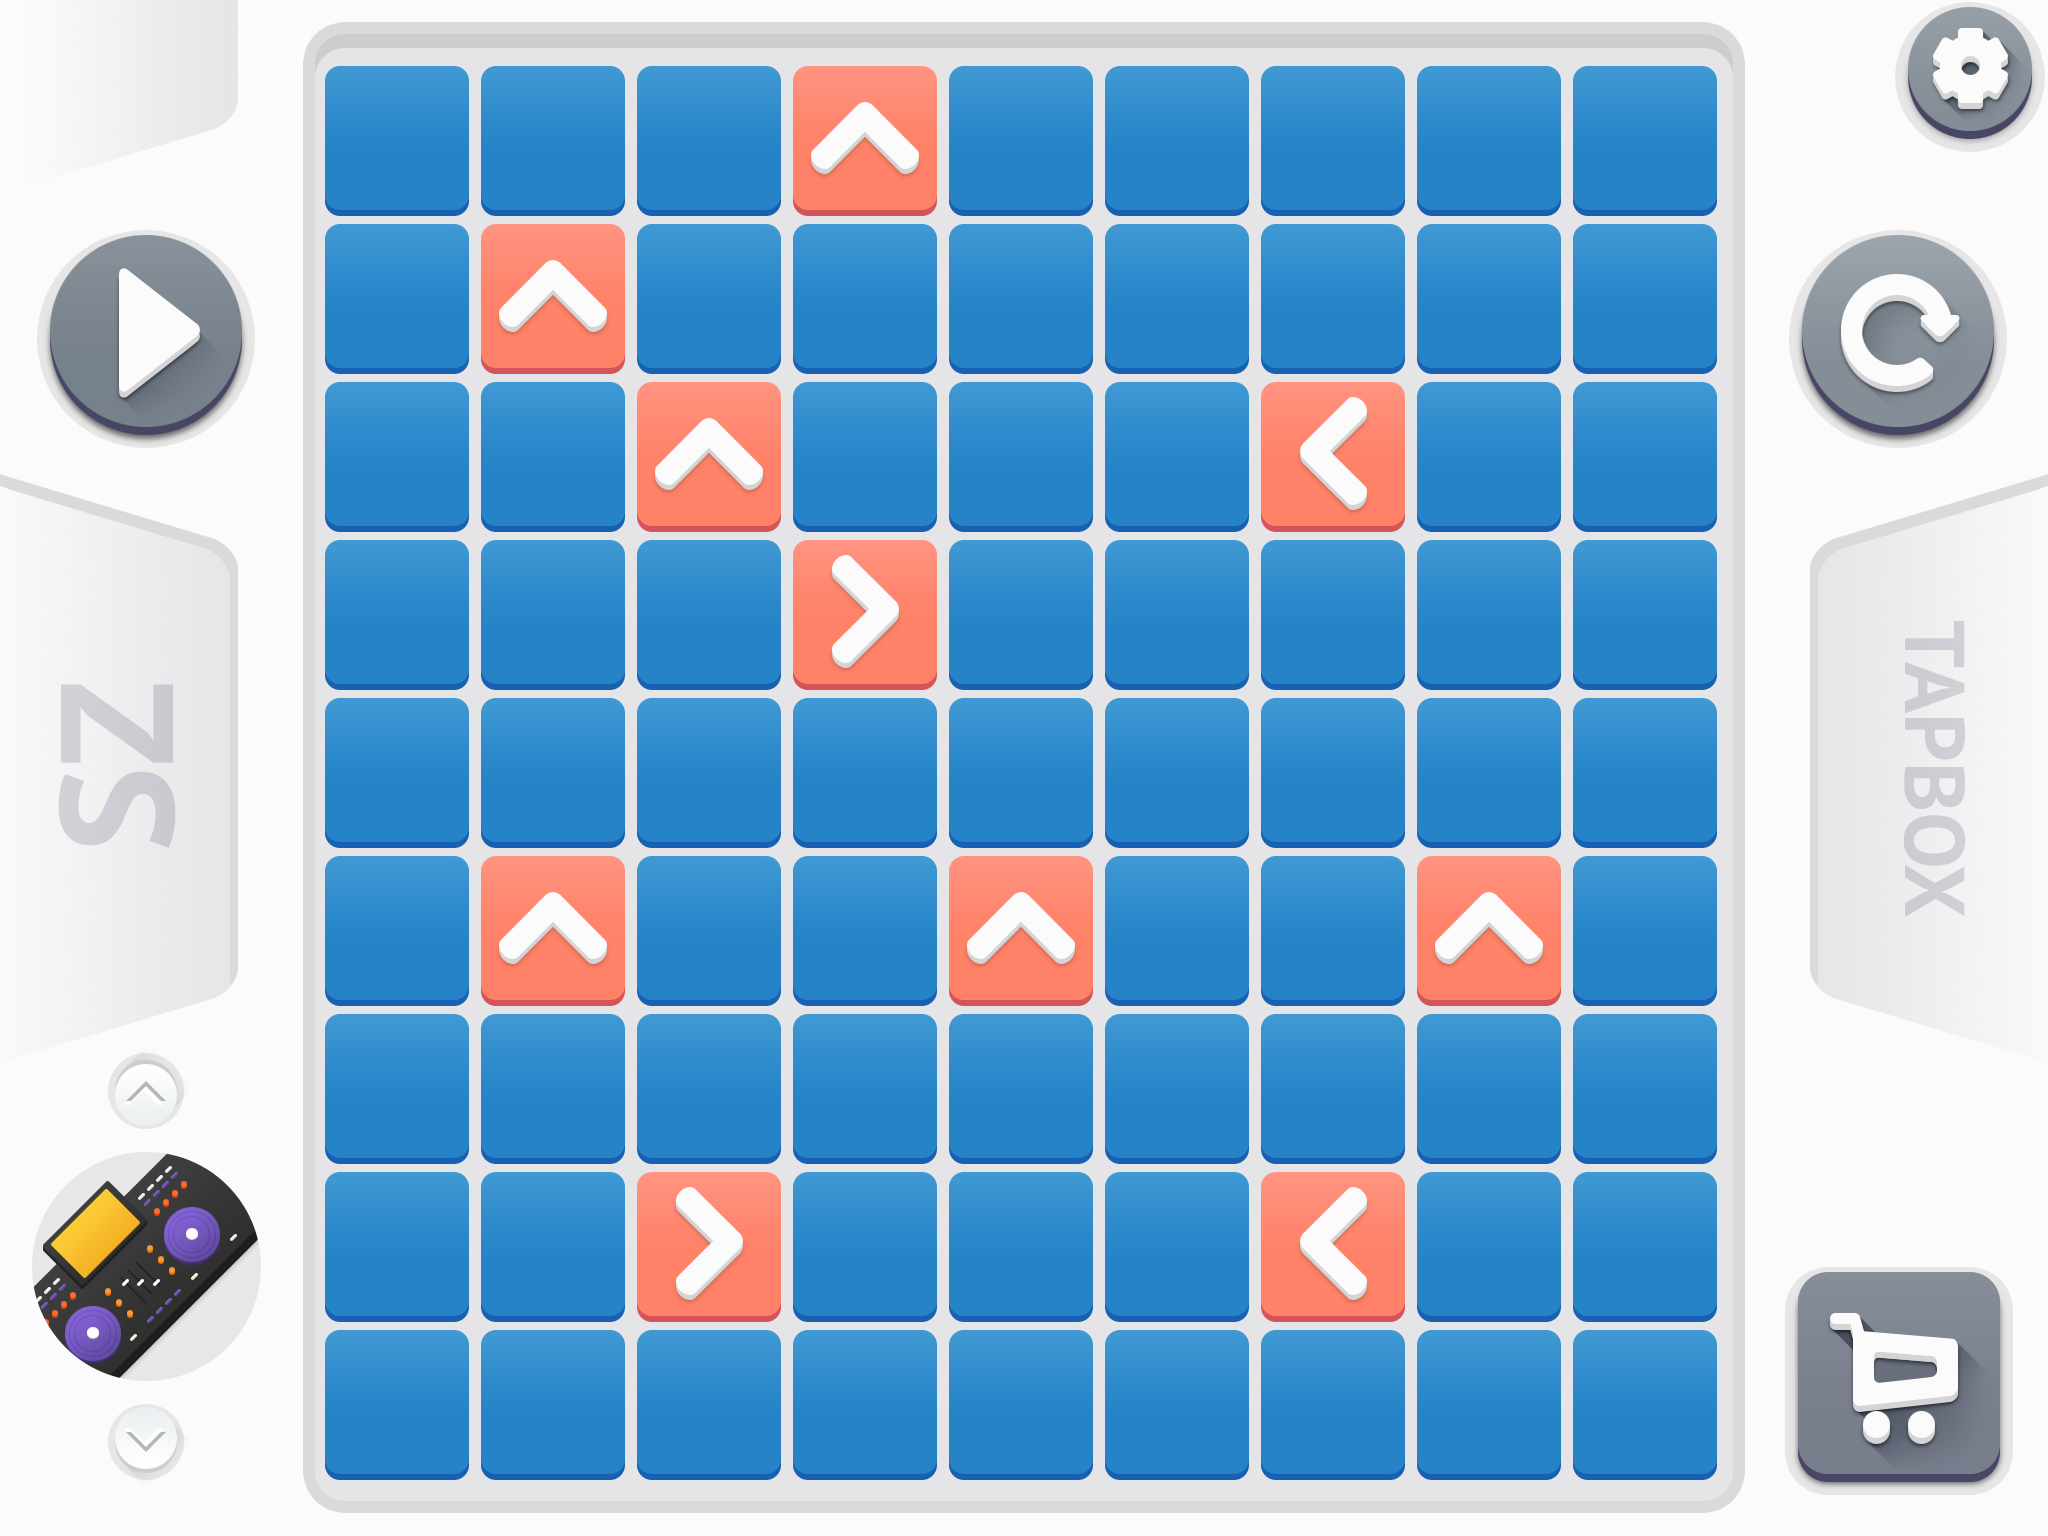
\includegraphics[width=12 cm]{images/SoundZen.PNG}
   \centering
   \caption{SoundZen: grid-based, right-to-left and discrete pitch layout}
   \label{fig: SoundZen}
 \end{figure}
 \bigskip

 However, not all the grid-based sequencer applications increase pitch from bottom to top. There is a small portion of sequencer increase pitch from left to right. For instance, SoundZenHD used a left-to-right pitch mapping (see figure: \ref{fig: SoundZen}).

In addition to the discrete pitch mapping, there are attempts to implement the continuous pitch. \textit{CSketch Lite} followed the classic grid-based layout, but it implements continuous sequencing (see Figure \ref{fig: CSketch}). By implementing the continuous sequenceing, \textit{CSketch Lite} is able to prodecue continuous sound in a series steps rather than make discrete sound step by step, which breaks the bound of the traditional music sequencer. Therefore, the pitch is changing continuously in \textit{CSketch Lite}. In figure \ref{fig: CSketch}, the yellow and blue line denote the trend of pitch changing. Take the top-left yellow line as an example, the pitch of the sound is continuously droping from G$\#$ to F. Even though, the pitch of the above music sequencer applications are still linear mapping.

Except for the linear mapping though the grids, some few Apps adopted the non-linear pitch mapping. For instance, \textit{Orbita} simulates the movemment of a small planet orbits around a central planet along an elliptical path. And in this case, different color of \textquotedblleft{planet}\textquotedblright represent different instruments, which produces sound while elliptical orbit. The pitch is changing continuously based on the distance between the small planet and the central planet(see figure \ref{fig: Orbita}).

\bigskip
\begin{figure}[h]
  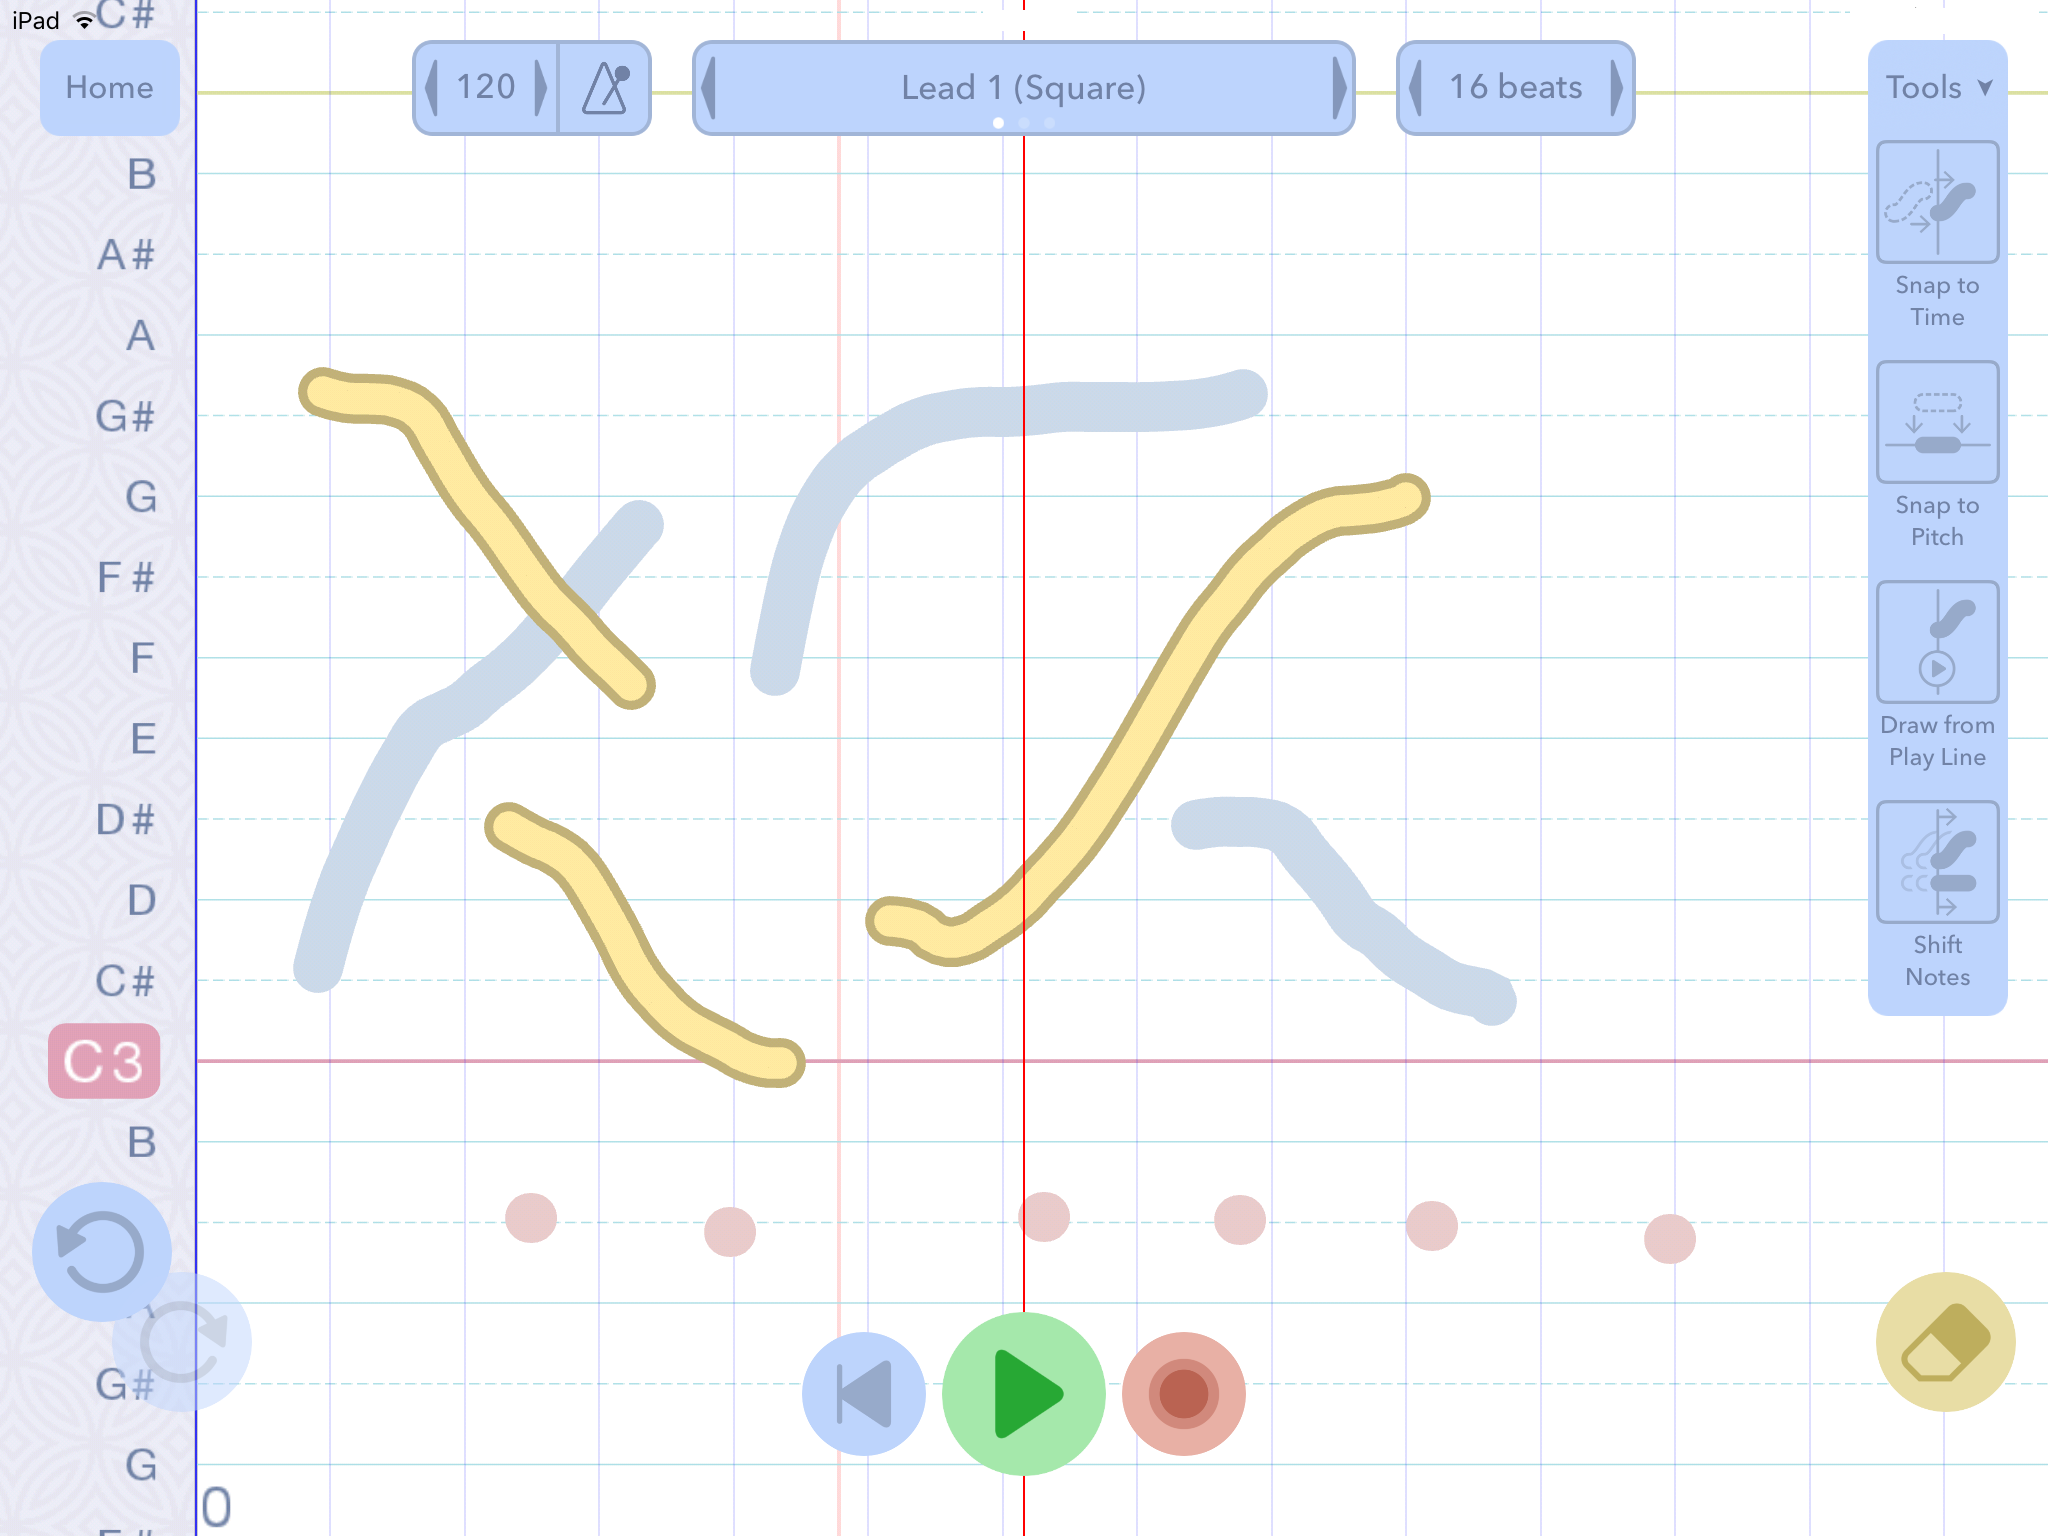
\includegraphics[width=12 cm]{images/CSketch_Lite.PNG}
  \centering
  \caption{CSketch Lite: grid-based, top-to-bottom and continuous pitch layout}
  \label{fig: CSketch}
\end{figure}
\bigskip

It is not unusal of mapping pitch to colour in music applications \citep{Reference14}. However, there was only one music sequencer found to represent pitch with different colors (see Figure \ref{fig: Volotic}). In \textit{Volotic}, there is an emiter which continuously emits red little dot sequently. The red color, in this case, means note C or \textbf{Do} which is the first note of the fixed-Do solfège scale. Once the red little dot passed though a tone assigner, it's tone changed relatively and so as it's color. In Figure \ref{fig: Volotic}, the green symbol is a tone assigner called TUNNING, and the number in the middle denotes what note it is going to assign. There are seven different TUNNINGs which together consist the key of C(or C major).

However, this color-based mapping is not intuitive. It takes significant effort to link different keys to colors. Besides, in this case, the two colors between pitch E (\textbf{Mi}, the third note of the C major scale) and pitch F (\textbf{Fa}, the fourth note of the C major scale) is very difficult to distinguish. This unintuitive mapping could be the reason why the color-based pitch is not widely implemented, and we will look into the details in the next chapter.

\textbf{Triggering and Timing.} In \citeauthor{Reference14}'s study, the mechanics of how users inteacted with applications and the methods of how time was represented were studied seperately. However, in most music sequencer applications, time is used to triiger sounds. Therefore, triggering and timing were analyzed together in our study.

Unsuperisingly, given the fact that toggles are primary used on sequencer hardware, virtual toggles are the most commonl method for users to control sequencer applications to start producing sounds. In Figure \ref{fig: Beatwave}, \ref{fig: SoundZen} and \ref{fig: CSketch} there are virtual toggles acting as main switch to control the play/stop operation. After the main switch turned on, time is uesd to determaine the triggering sequence of a series of notes or several pieces of sounds. Likewise, timing in the majority of sequencer applications follow the convention of sequencer hardware, which time move from left to right. Some very few applications don't have an explicity display of time, such as \textit{Orbita} and \textit{Volotic} (see Figure \ref{fig: Orbita}, \ref{fig: Volotic}).

\textbf{Timber and Volumn}The majority of music sequencer applications use toggles to change timbers and volumn. Normally, there are several preset timbers and users can shifted between different timbers by selecting one of the preset timbers. Only a very small number of applications use additional control over timber. \textit{Volotic} uses the the symbol of different instruments to represent the unique timbers (see Figure \ref{fig: Volotic}. Essentially, it is still a toggle but in a twisted form.

\bigskip
\begin{figure}[h]
  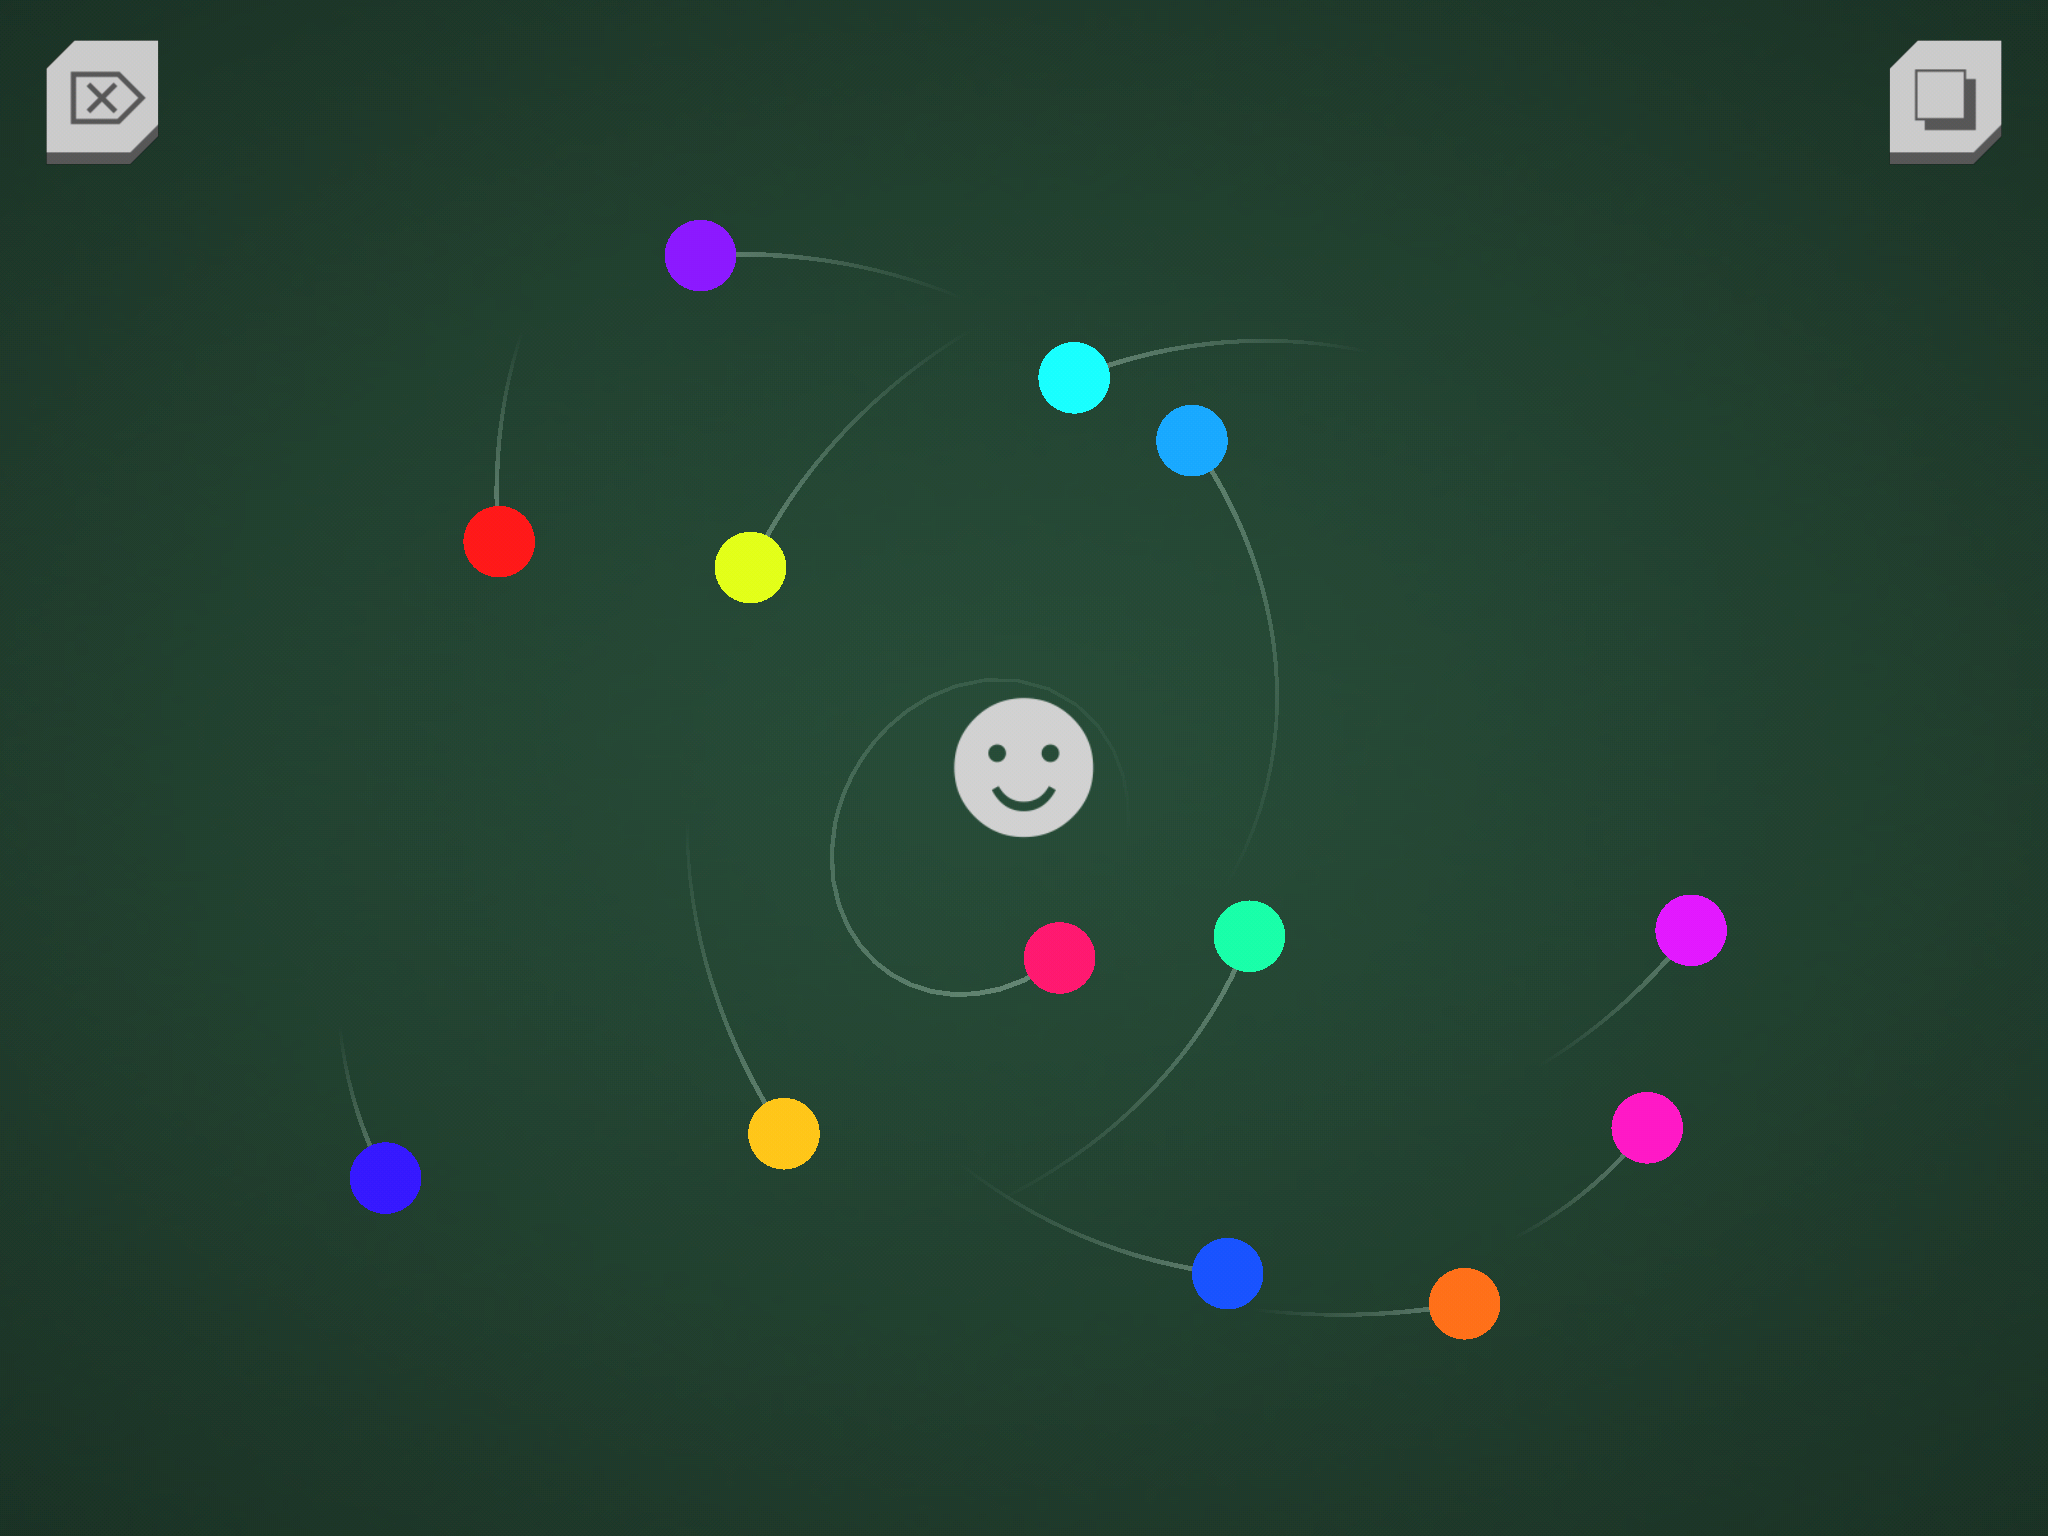
\includegraphics[width=12 cm]{images/Orbita.PNG}
  \centering
  \caption{Orbita: elliptical orbita, non-linear and continuous pitch layout}
  \label{fig: Orbita}
\end{figure}
\bigskip

The reason why mapping of volumn is combined with timber is the majority of music sequencer use the same mapping which is a slider or toggle. Other volumn controls are very rare. \textit{Orbita} is the only example of using the distance between the satellite and the planet to control the volumn. The volumn is turn up when satellite get close to the central planet. Conversely, the volumn goes down when two planets move apart.

\bigskip
\begin{figure}[h]
  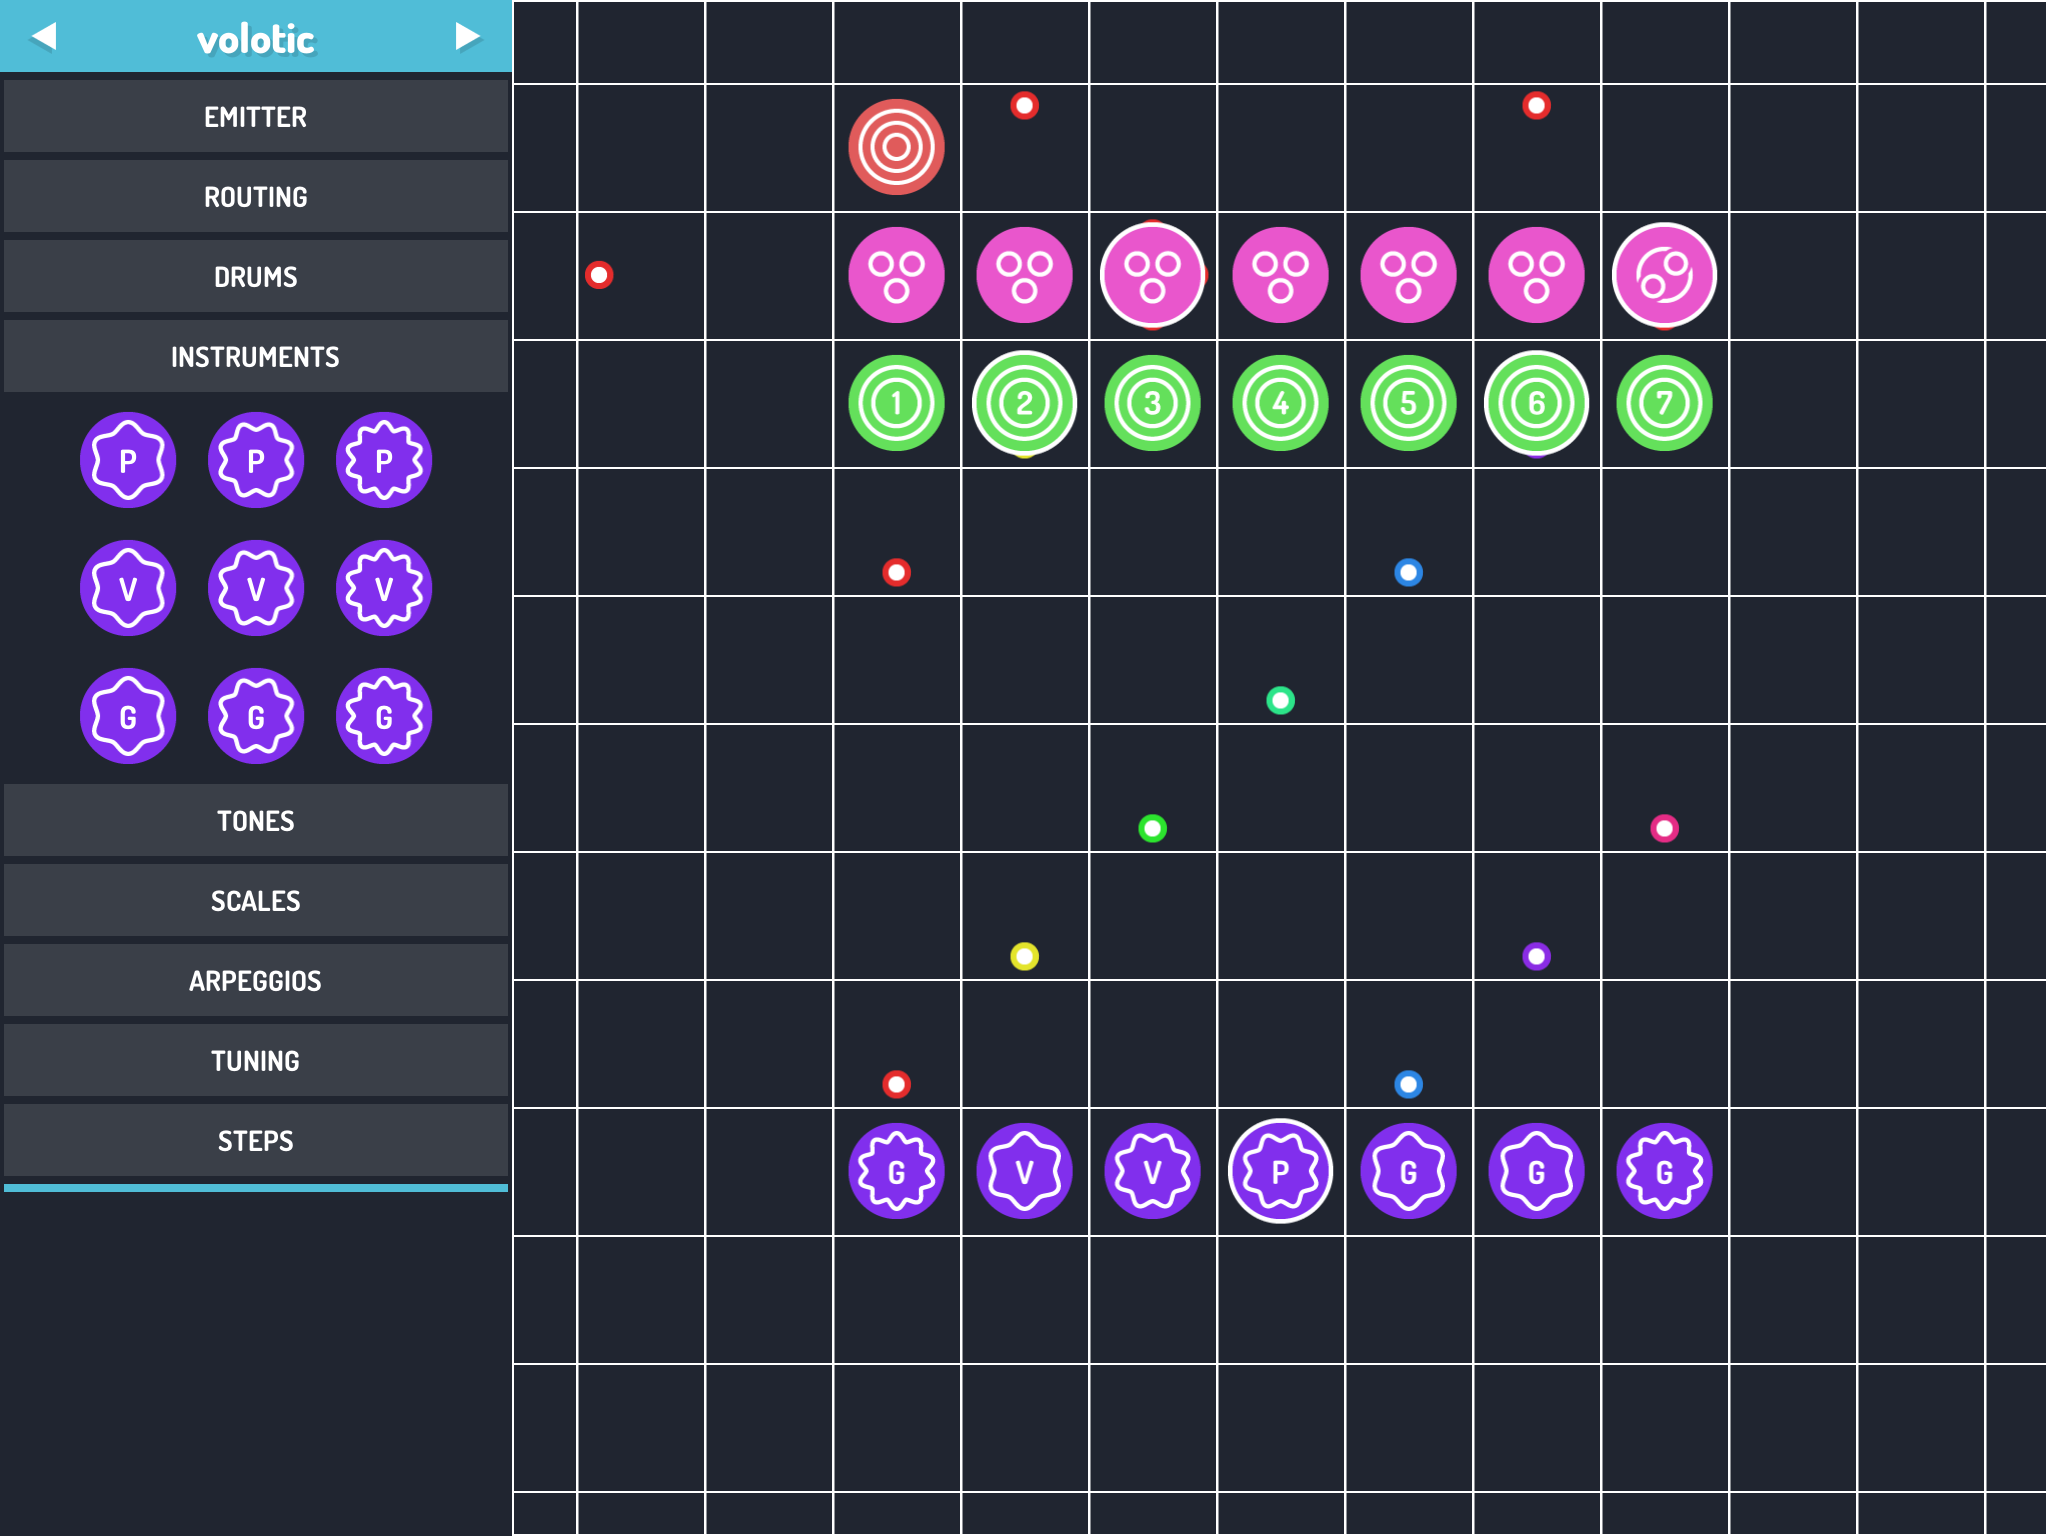
\includegraphics[width=12 cm]{images/Volotic.PNG}
  \centering
  \caption{Volotic: game-like, linear and color-based pitch layout}
  \label{fig: Volotic}
\end{figure}
\bigskip

\section{Results}

According to the three main classification crterias, we seperated the 

\label{sec: result}
\bigskip
\begin{figure}[h]
  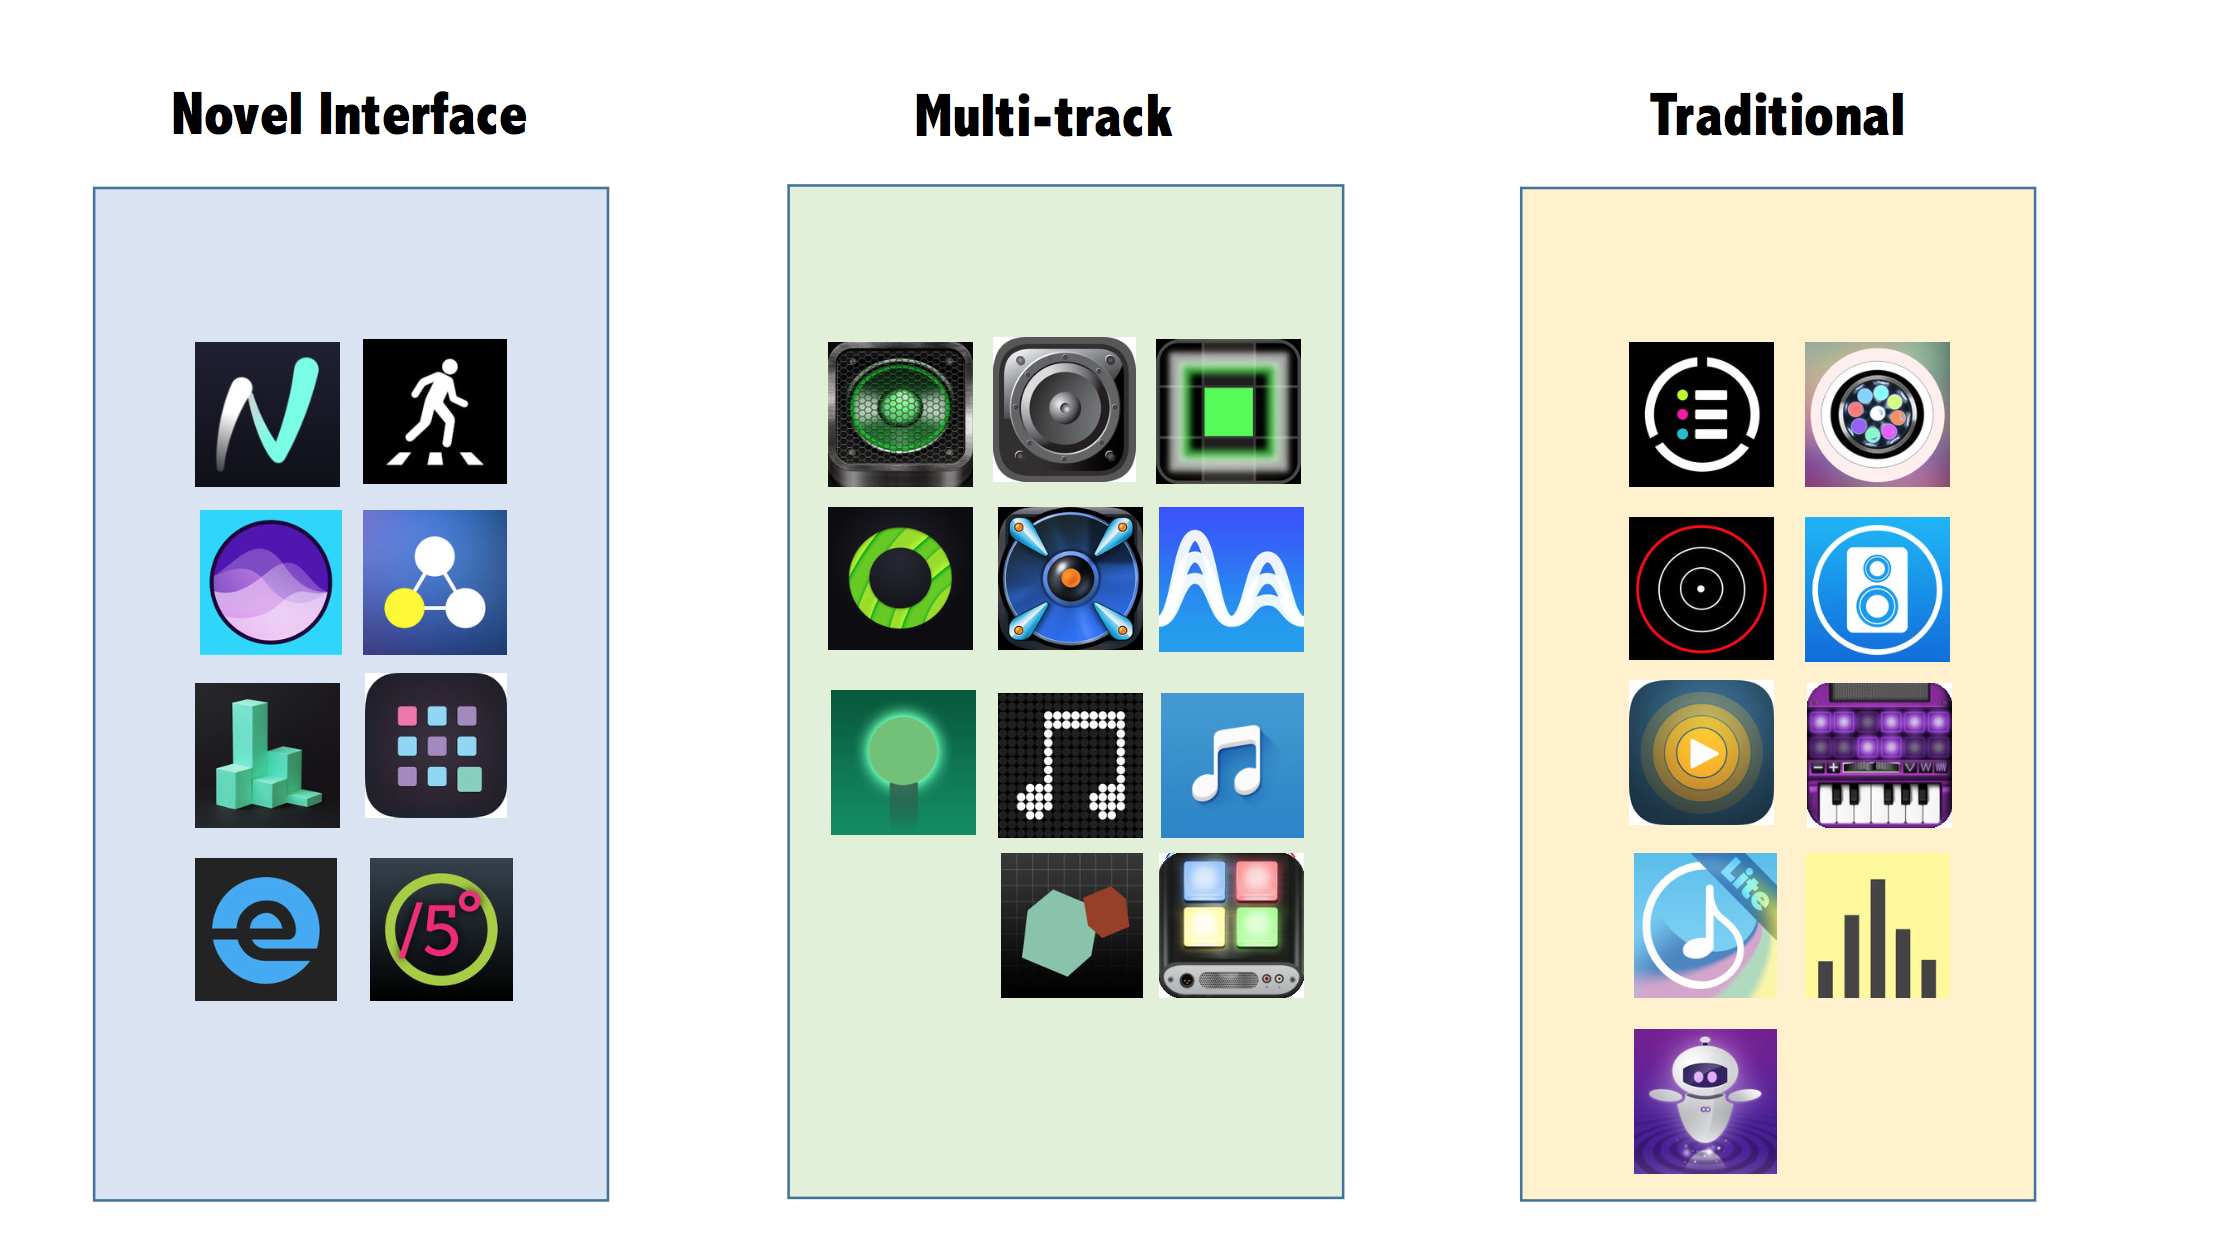
\includegraphics[width=\textwidth]{images/Template.png}
  \centering
  \caption{This is how result of study one going to look like}
  \label{fig: Results}
\end{figure}
\bigskip

\bigskip
\begin{figure}[h]
  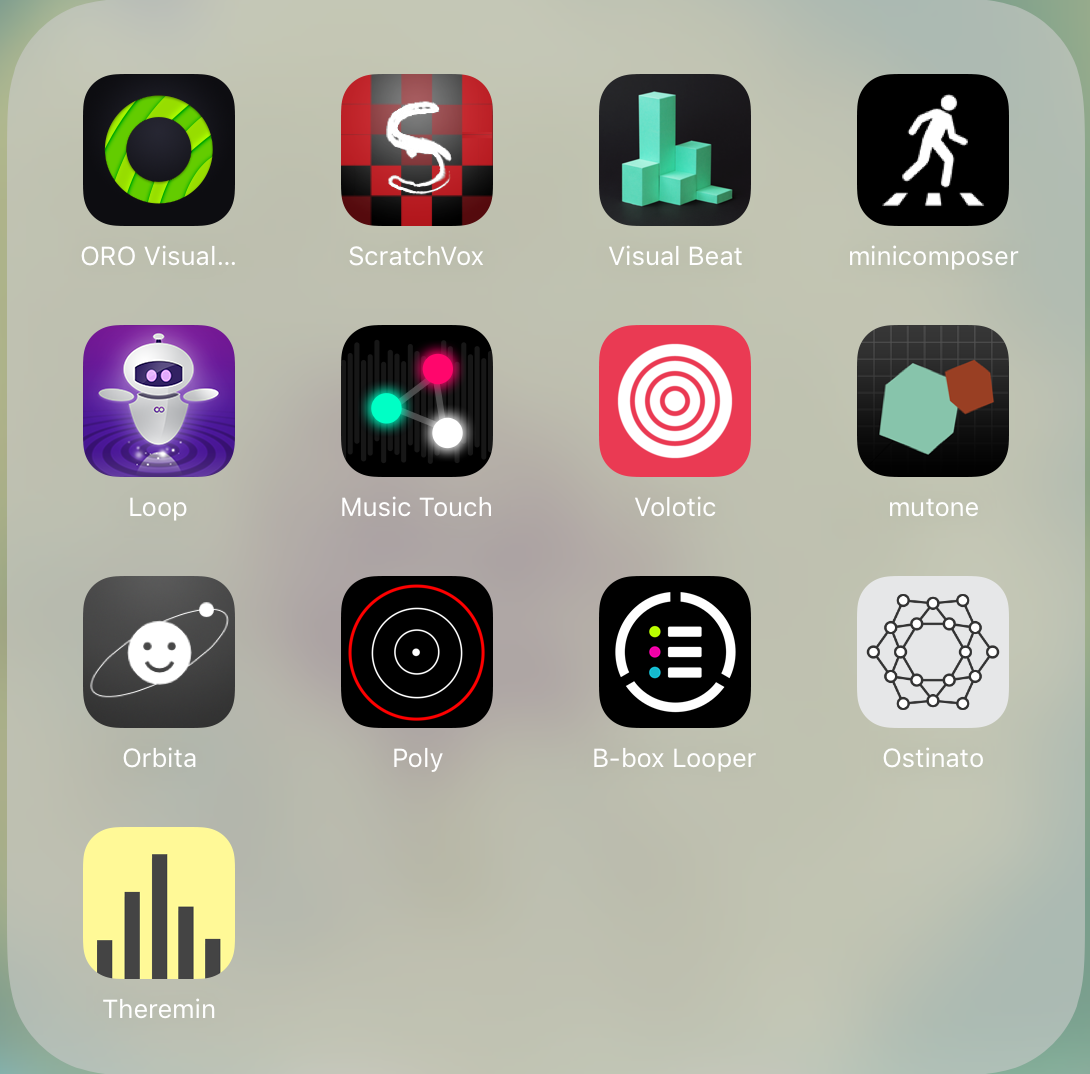
\includegraphics[width=0.5\textwidth]{images/Novel.png}
  \centering
  \caption{Apps under the Novel category}
  \label{fig: Novel}
\end{figure}
\bigskip

\bigskip
\begin{figure}[h]
  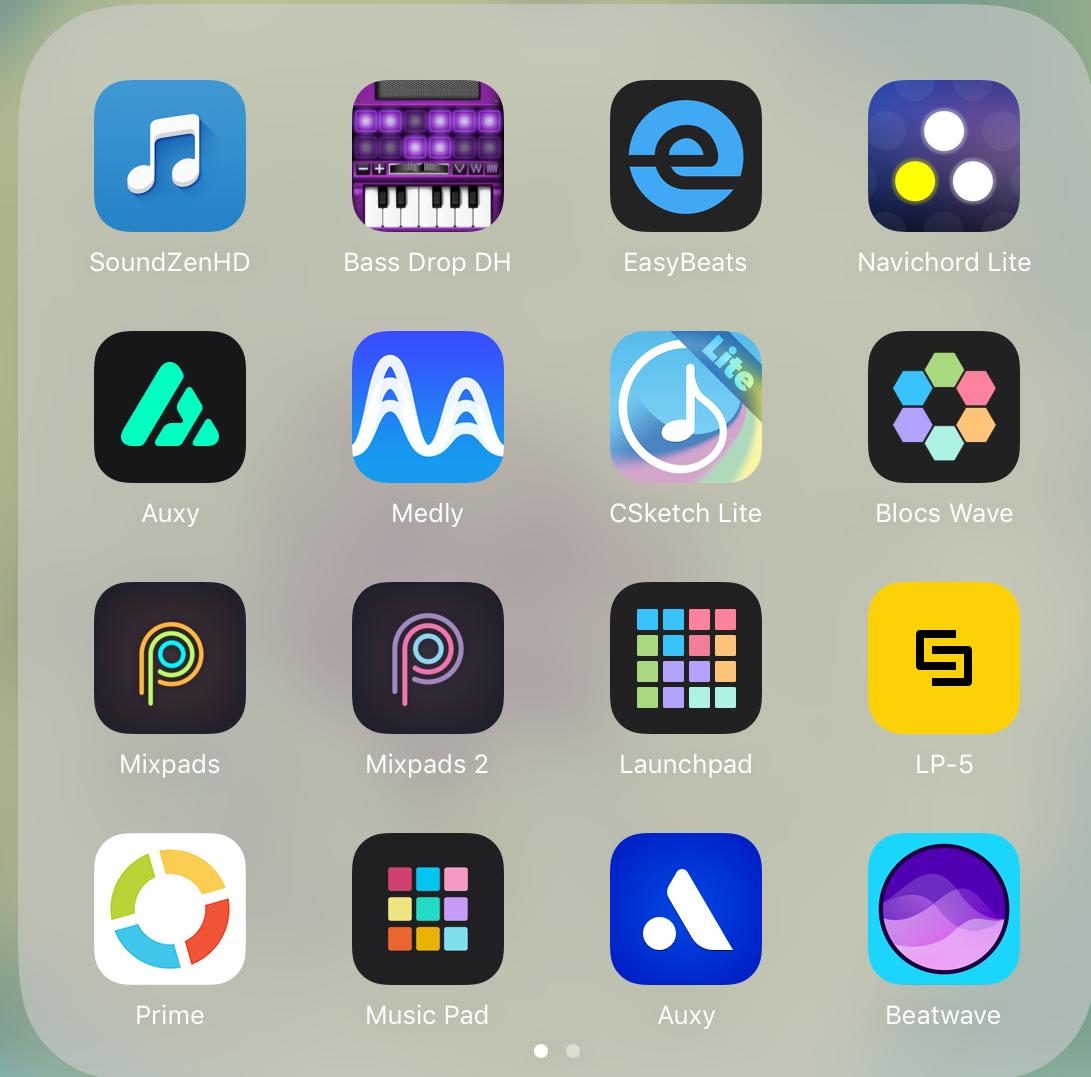
\includegraphics[width=0.505\textwidth]{images/Multi-track2.png}
  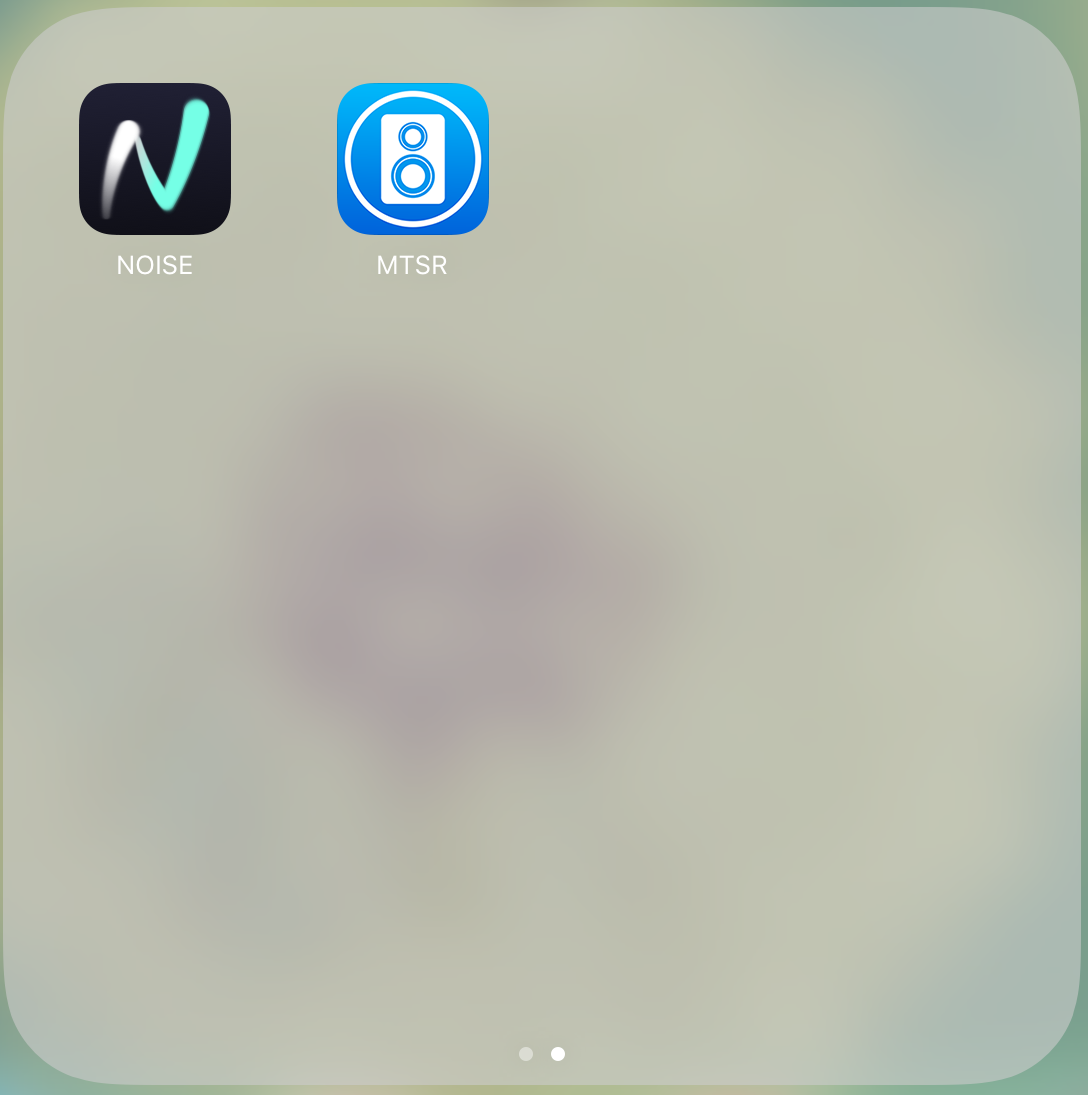
\includegraphics[width=0.495\textwidth]{images/Multi-track1.png}
  \caption{Apps under the Multi-track category}
  \label{fig: Multi}
\end{figure}
\bigskip

\bigskip
\begin{figure}[h]
  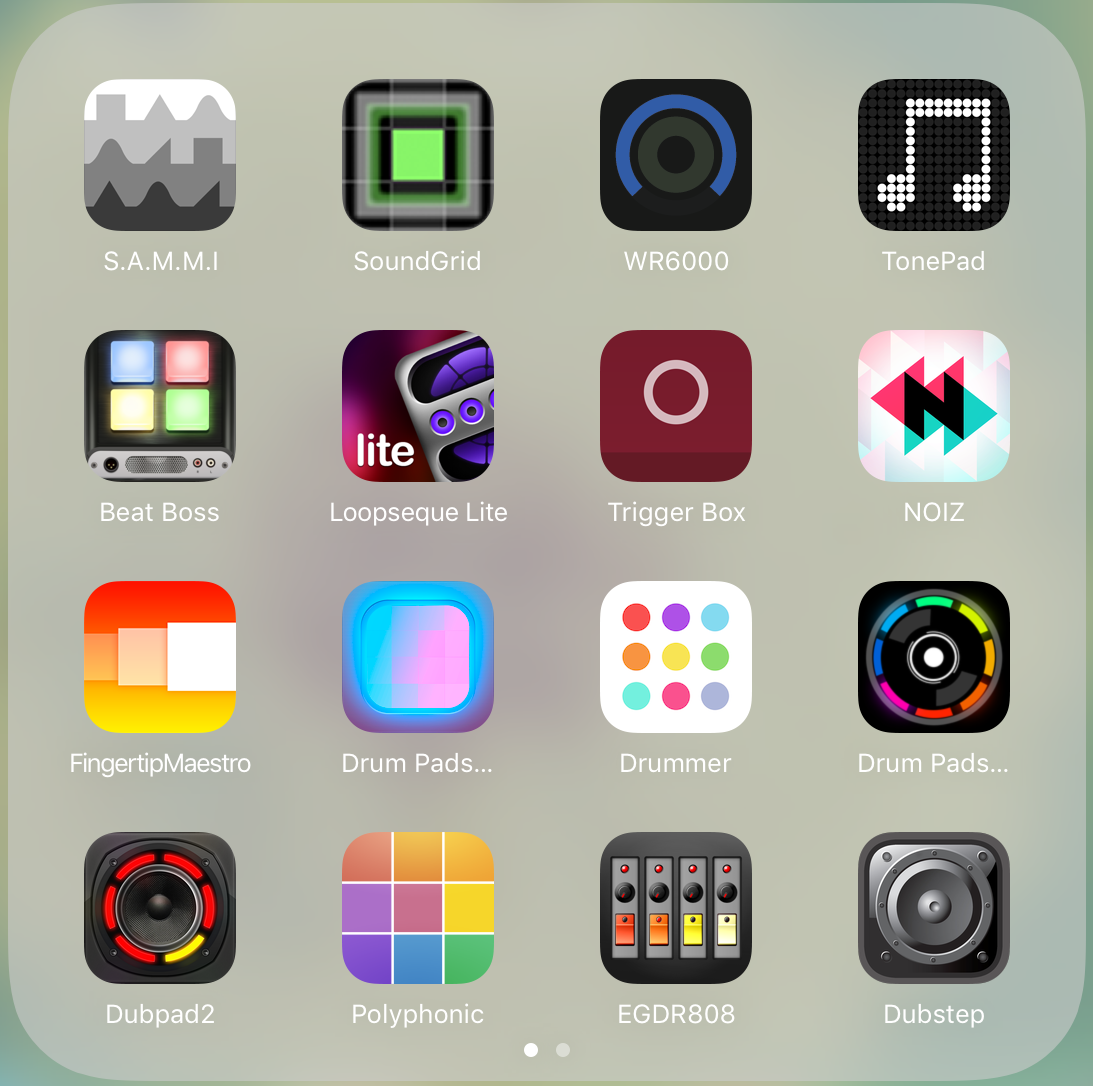
\includegraphics[width=0.50\textwidth]{images/Traditional1.png}
  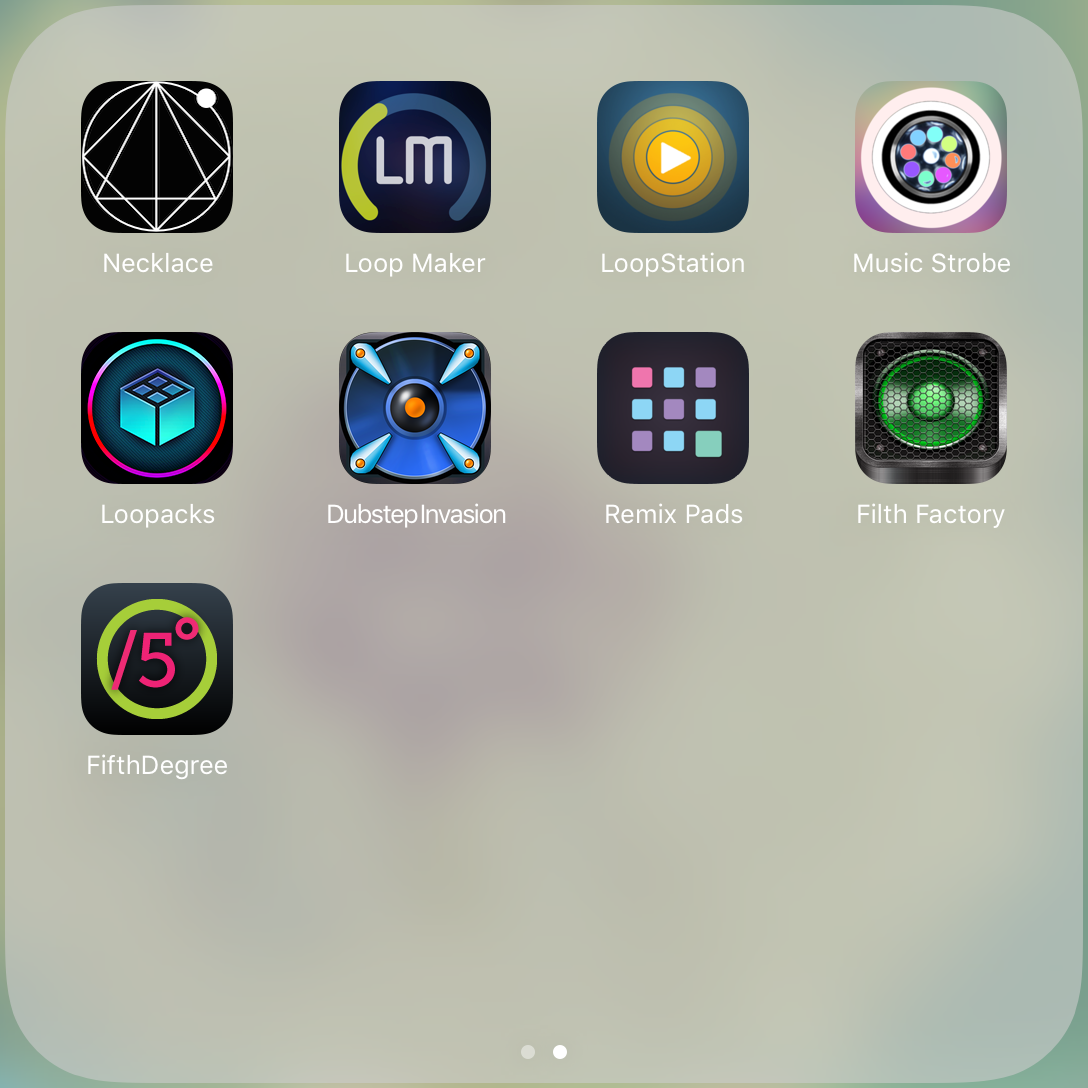
\includegraphics[width=0.50\textwidth]{images/Traditional2.png}
  \caption{Apps under the Traditional category}
  \label{fig: Traditional}
\end{figure}
\bigskip
 % Experimental Setup

%\chapter{Study 2: User Study}

Following the first study (See Chapter \ref{ch: chapter 3}), A laboratory study was conducted to justify user experience on different design patterns of music sequencers. Base on the previous work of evaluating music instruments, a questionnaire was designed to measure muscians experience (See Section \ref{subsec: questionnaire}).

\section{Method}
\subsection{Questionnaire}
\label{subsec: questionnaire}

Base on \citeauthor{Reference0}'s work, which developed a 80-item pool ordered by descending mean importance for questionnaire, 10 questions that scored the highest mark from 9 different categories were used in the user study (see Appendix \ref{app:Appendix A}). 

\subsection{Interview}

\section{Participants}



\section{Results}

\section{Discussion}

\section{Summary}
 % Experiment 1

%\pagestyle{fancy}
\rhead{\thepage}
\lhead{Conclusion}
\chapter{Conclusion}
\label{ch: chapter 5}

This thesis has described studies that have been conducted to evaluating the touch-based music sequencer apps on iPad. In Chapter \ref{ch: chapter 2}, we illustrated the background of DMIs and highlighted the fact of apparent popularity of mobile devices. Also, we introduced the development of NIME community and current situation of evaluating the newborn musical interface. Then we carried out two consecutive studies to investigate factors that affect music sequencer interface's expressivity, control and aesthetics. In the first study, we examined 55 music sequencer downloaded from App Store. Results of the first study presented an interface taxonomy of current sequencer apps on iOS App Store (see Chapter \ref{ch: chapter 3}). And in the second study, followed by the interface taxonomy we concluded in the previous chapter, we perfomed an HCI user study with twenty musicians of the selectedapplications. We summarized the influence of different design appoachon on music sequencer interface (see Chapter \ref{ch: chapter 4}).

Through the evaluation of music sequencer on iPad, we identified the following contributions: \\
\qquad$\bullet$ An interface taxamony of music sequencer apps based on the mapping of interaction has been created, and which can potentially benefit future study on classifying touch-based musical interface on iPad or other similar mobile devices.\\
\qquad$\bullet$ Conducting an HCI user study and present an example questionnaire for analyzing musical interface on mobile devices.\\
\qquad$\bullet$ Providing design guidelines for future music sequencer development.

\section{Limitation and Future Work}

Associated with the contribution there are some limitations with the research. We only collected music sequencer applications from the iOS App Store. There are still more similar apps developed for Android OS have not been stuied.
The various music background of participants may affact their judgement on single senquencer apps. Last but not least, in the user study, we only analyzed the musicians opinions from a short impression.

Future work may expand the study object to Android applications, and further investigate the music sequencer interface from a long time study.



% \section{Future Work}
%
% Design guidline
% Develop our own sequencer
% Further investigate other music instrument application on the App Store by employing the user study.


\clearpage
 % Experiment 2

%\input{Chapters/Chapter6} % Results and Discussion

%\input{Chapters/Chapter7} % Conclusion

%% ----------------------------------------------------------------
% Now begin the Appendices, including them as separate files

\addtocontents{toc}{\vspace{2em}} % Add a gap in the Contents, for aesthetics

\appendix % Cue to tell LaTeX that the following 'chapters' are Appendices

\chapter{App Store Music Sequencer Applications}

\begin{tabular}{ |p{3cm}||p{3.5cm}|p{3.5cm}|p{3.5cm}||}
 \hline
 \multicolumn{4}{|c|}{App Store Music Sequencer Applications} \\
 \hline
 Application Name   & Description  & Seller & Link\\
 \hline
 Music Pad  & dj player remix electronic music beat & Xinggui Zhang & \url{<https://appsto.re/au/_Dkmeb.i>}\\

 Volotic & N/A & Scott Garner &
\url{ https://appsto.re/au/-WW64.i}\\

 Beatwave & N/A & collect3 &
 \url{https://appsto.re/au/UzERv.i}\\

 EGDR808 & Drum Machine free & Elliott Garage &
 \url{https://appsto.re/au/rPfXO.i}\\

 LoopStation & N/A & Rene Zuidhof &
 \url{https://appsto.re/au/UzMw7.i}\\

 Noise & N/A & ROLI Ltd &
 \url{https://appsto.re/au/Zzkr8.i}\\

 Music Strobe Starter & N/A & Arun Bab&
 \url{https://appsto.re/au/y4NFQ.i}\\

 Beatbox Looper & N/A & Pierre Guilluy&
 \url{https://appsto.re/au/Sfk6R.i}\\

 Dubstep Invasion & Music And Song Hit Maker & Jochen Heizmann&
 \url{https://appsto.re/au/Oane3.i}\\



 \hline
\end{tabular}
\fancyfoot[C]{\thepage}

\newpage
\pagestyle{fancy}
\fancyhead[L]{Appendix A}
\fancyfoot{}
\fancyfoot[C]{\thepage}

\begin{tabular}{ |p{3cm}||p{3.5cm}|p{3.5cm}|p{3.5cm}||}
 \hline
 \multicolumn{4}{|c|}{App Store Music Sequencer Applications(Continued)} \\
 \hline
 Application Name   & Description  & Seller & Link\\
 \hline

 Remix Pads & make groove beats record music app & Alexey Natarov&
 \url{https://appsto.re/au/R7_pdb.i}\\

 Music Touch & Make Mix Music DJ Beats & Qiao He&
 \url{https://appsto.re/au/D_ZTdb.i}\\

 Loop maker & Amazing music maker & Miguel Saldana &
 \url{https://appsto.re/au/MpDthb.i}\\

 Drum Pads Machine & Beat maker dj music studio & Alexey&
 \url{https://appsto.re/au/JZ9adb.i}\\

 Drum Pads Machine 2 & Beat maker dj music app & Alexey Natarov&
 \url{https://appsto.re/au/c5DZdb.i}\\

 MIxpads & Virtual dj pads sampler free app & Alexey Natarov &
 \url{https://appsto.re/au/CPj1eb.i}\\

 Loopacks & Music Maker Loop Machine DJ Beats & Hernan Arber &
 \url{https://appsto.re/au/oXKt1.i}\\

 Dubstep Dubpad 2 & Electronic Music Sampler & FAD Games LLC &
 \url{https://appsto.re/au/mCRXO.i}\\

 NOIZ & Make Epic Music & Studio Amplify &
 \url{https://appsto.re/au/KK9Uab.i}\\

 Blocs Wave & Make Record Music & Novation &
 \url{https://appsto.re/au/L0MTab.i}\\

 MIxpads 2 & Dubstep Trap drum pad sampler for DJ & Alexey Natarov &
 \url{https://appsto.re/au/oH_ffb.i}\\

 Polyphonic! & NA & Flip Studios LLC &
 \url{https://appsto.re/au/u_PhS.i}\\

 Steve Reich's Clapping Music & Improve Your Rhythm & Amphio Limited &
 \url{https://appsto.re/au/R-JA4.i}\\

 Music Pad  & remix electronic music beat & Xinggui Zhang &
 \url{https://appsto.re/au/_Dkmeb.i}\\

 Loop Community & NA & Loop Community &
 \url{https://appsto.re/au/VyLNN.i}\\

 LP-5 & Loop-based Music Sequencer & Markus Waldboth &
  \url{https://appsto.re/au/Z6EDN.i}\\

  \hline
 \end{tabular}

 \newpage
 \pagestyle{fancy}
 \fancyhead[L]{Appendix A}
 \fancyfoot{}
 \fancyfoot[C]{\thepage}

 \begin{tabular}{ |p{3cm}||p{3.5cm}|p{3.5cm}|p{3.5cm}||}
  \hline
  \multicolumn{4}{|c|}{App Store Music Sequencer Applications(Continued)} \\
  \hline
  Application Name   & Description  & Seller & Link\\
  \hline

 Dubstep Song Construction Kit &NA & Jochen Heizmann &
  \url{https://appsto.re/au/Knd0I.i}\\

 Dubstep Filth Factory & Sampler and Loop Machine & Ben Frost &
  \url{https://appsto.re/au/iHnUX.i}\\

 Monolith Loop & Relax Meditate Sleep Zen & Monolith Interactive Inc.&
  \url{https://appsto.re/au/vfGDy.i}\\

 Theremin Synth & Loop Record Download & Luke Phillips &
 \url{https://appsto.re/au/gJI2bb.i}\\

 Music Makr JAM & Create remix share your music! & JAM just add music GmbH &
 \url{https://appsto.re/au/EXEG0.i}\\

 Novation Launchpad & Make Remix Music & Novation &
 \url{https://appsto.re/au/QNk1I.i}\\

 Multi Track Song Recorder & NA & Derrick Walker &
 \url{https://appsto.re/au/Ygbsx.i}\\

 Triqtraq & Jam Sequencer music making on the go & Zaplin Music &
 \url{https://appsto.re/au/G8XhD.i}\\

 Trigger Box & NA & Justus Kandzi &
 \url{https://appsto.re/au/j4Hn1.i}\\

 Composer's Sketchpad Lite & NA & Alexei Baboulevitch &
 \url{https://appsto.re/au/nWJO_.i}\\

 Orbita for iOS & NA & Keijiro Takahashi&
 \url{https://appsto.re/au/kBIaN.i}\\

 S.A.M.M.I. & NA & Christopher Ayles &
 \url{https://appsto.re/au/YDMeY.i}\\

 ScratchVOX & NA & ScratchVOX &
 \url{https://appsto.re/au/e4aX0.i}\\

 Oro & Visual Music & Light the Music LLC &
   \url{https://appsto.re/au/d6px5.i}\\

 Poly & NA & James Milton &
   \url{https://appsto.re/au/LFspN.i}\\

 Mutone & NA & william LINDMEIER &
   \url{https://appsto.re/au/IkoJM.i}\\

  \hline
 \end{tabular}

\newpage
\pagestyle{fancy}
\fancyhead[L]{Appendix A}
\fancyfoot{}
\fancyfoot[C]{\thepage}

 \begin{tabular}{ |p{3cm}||p{3.5cm}|p{3.5cm}|p{3.5cm}||}
  \hline
  \multicolumn{4}{|c|}{App Store Music Sequencer Applications(Continued)} \\
  \hline
  Application Name   & Description  & Seller & Link\\
  \hline

  WR6000 & NA & WEJAAM &
  \url{https://appsto.re/au/pM3E3.i}\\

  SoundZen HD & NA & Tapbox LTD &
  \url{https://appsto.re/au/dHrZB.i}\\

  SoundGrid & NA & Vitaly Pronkin &
  \url{https://appsto.re/au/fSB3s.i}\\

  Visual Beat & Interactive Music Video & Max Moertl &
  \url{https://appsto.re/au/B-8l6.i}\\

  MINI-COMPOSER & NA & Masayuki Akamatsu &
  \url{https://appsto.re/au/Ar8Ez.i}\\

 Loopseque Lite & NA & Casual Underground &
 \url{https://appsto.re/au/BTm8x.i}\\

 Bass Drop & Deep House Electronic music sampler and synthesizer & Ben Frost &
 \url{https://appsto.re/au/k3rp0.i}\\

 Beat Boss & Electronic Dance Music Sampler & Ben Frost &
 \url{https://appsto.re/au/DWLyU.i}\\

 TonePad &NA& LoftLab &
 \url{https://appsto.re/au/nOx1s.i}\\

 Navichord Lite & intuitive chord sequencer & Denis Kutuzov &
 \url{https://appsto.re/au/kTci2.i}\\

 EasyBeats Drum Machine Free MPC & Hopefully Useful Software & Christian Inkster &
 \url{https://appsto.re/au/gJ1Ot.i}\\

 Fifth Degree & MIDI Sequencer & Bernie Maier &
 \url{https://appsto.re/au/qFZM1.i}\\

 Light Medley & NA & Tek Min Ewe &
 \url{https://appsto.re/au/FU06hb.i}\\

 Medly &  Music Maker & Medly Labs Inc &
 \url{https://appsto.re/au/CP1c4.i}\\

 \hline
\end{tabular}
	% Appendix Title

%\chapter{Questionnaire}
\label{app: Appendix B}
% \pagestyle{fancy}
\fancyhead[L]{Appendix B}

% \begin{document}
\vspace{-1.8cm}
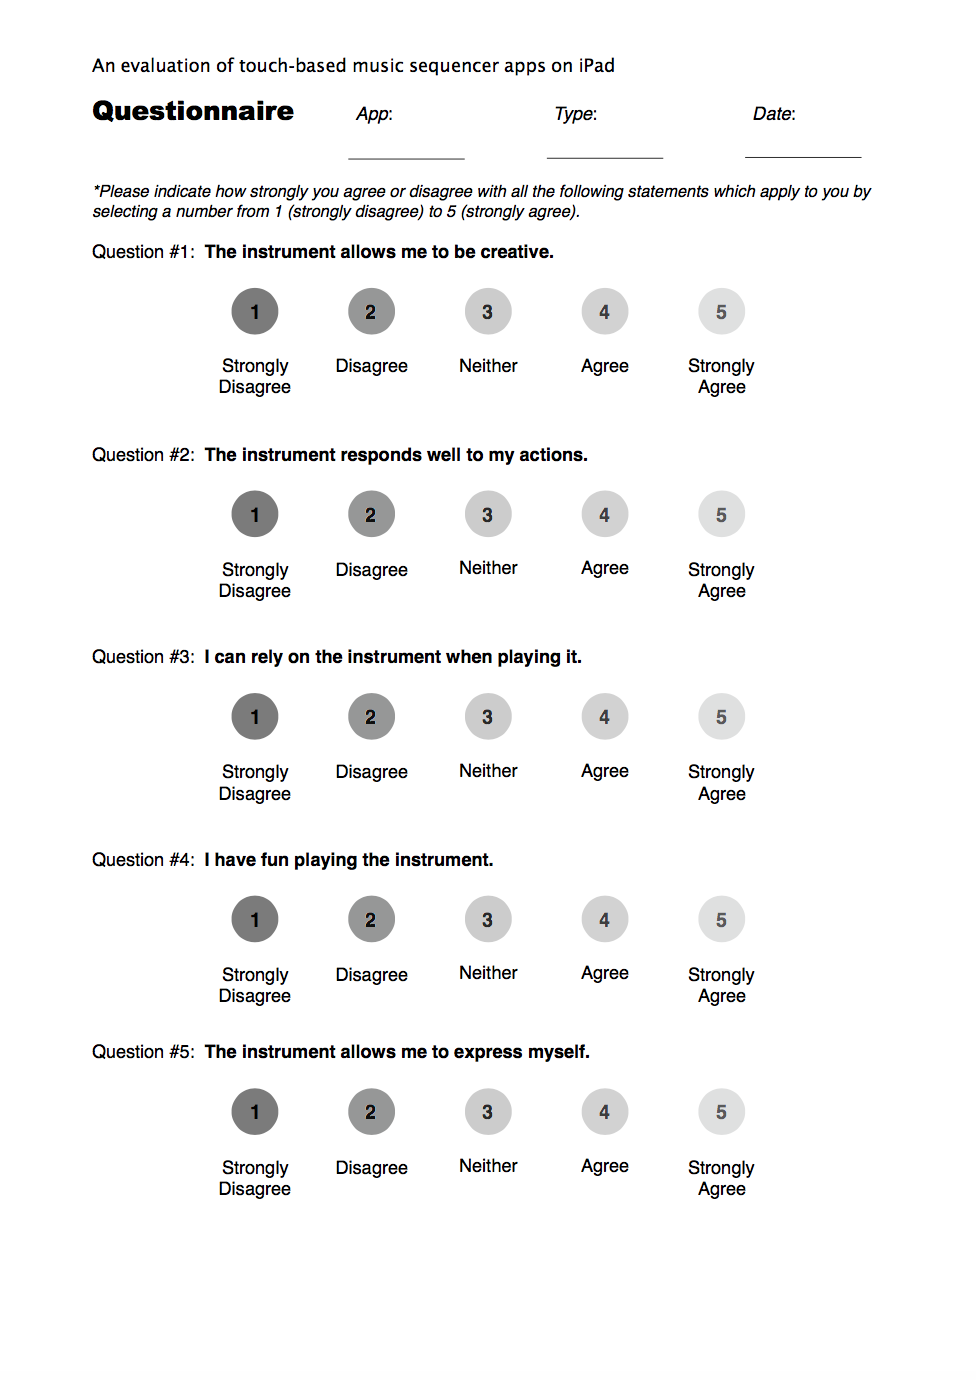
\includegraphics[width=\textwidth]{Questionnaire_1.png}

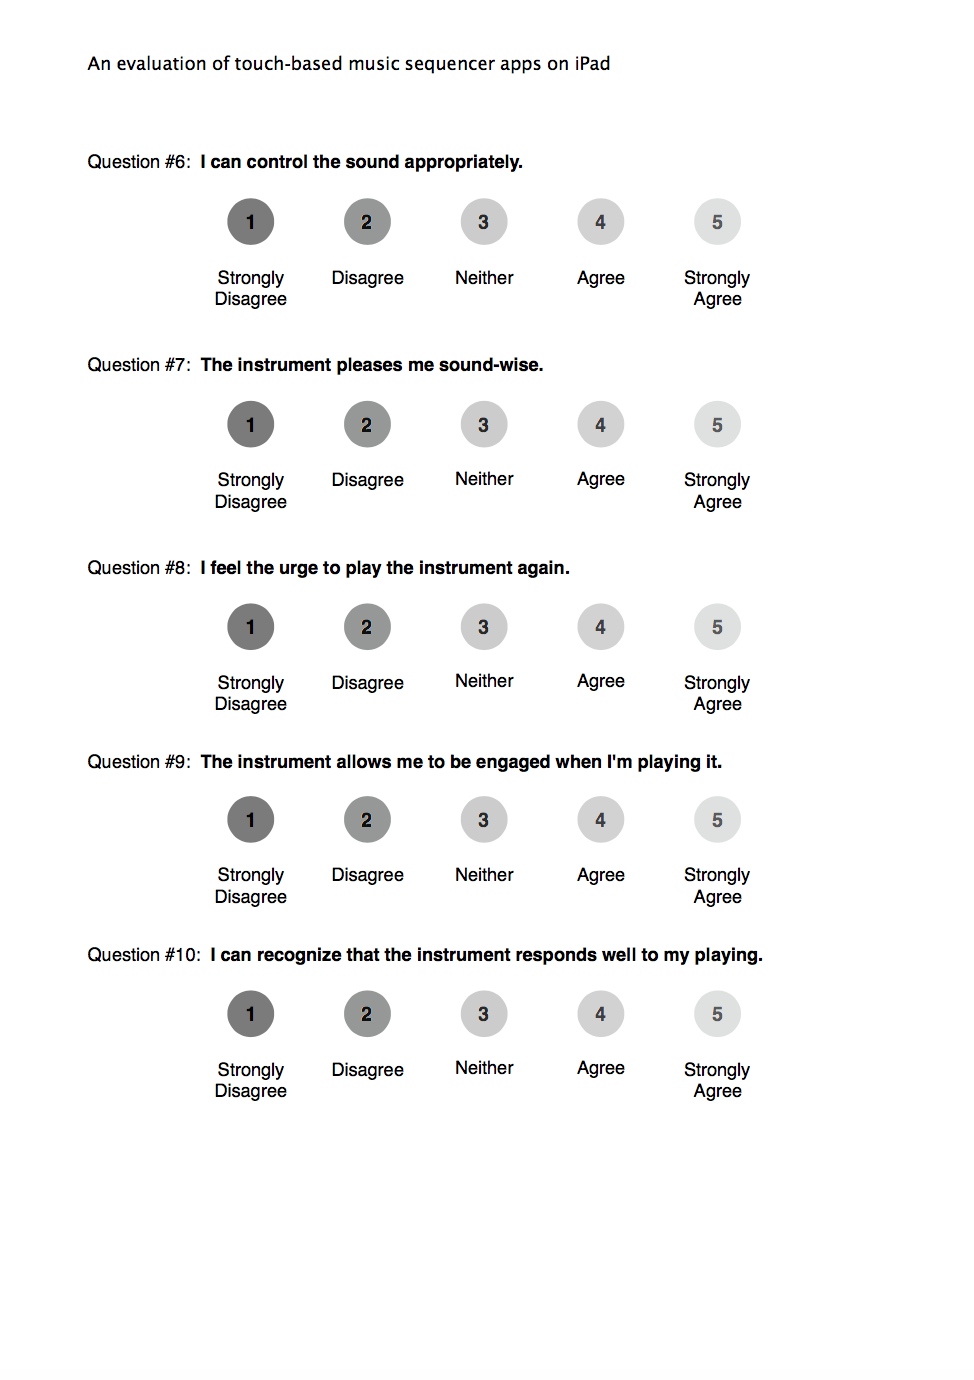
\includegraphics[width=\textwidth]{Questionnaire_2.png}
% \end{document}
 % Appendix Title

%\chapter{Interview Questions}
\label{app: AppendixC}
\fancyhead[L]{Appendix C}

This document contains a list of questions that will be asked in the interview.

{\fontfamily{qcr}\selectfont
1. Can you tell me about your experience and training in music? How long have you been learning? \\

2. What kind of instrument you play most in your spare time, and what kind of instrument you instrument you prefer to play? \\

3. Among the 3 apps you just played, do you find one app attracted you most, or you think they are all very boring? \\

4. Have you heard about or used music sequencers before? \\

5. After playing the three apps, can identify any interface patterns in these music sequencer apps? \\

6. Did one particular interface most inspired your creativity? How? \\

7. Do you think the complexity of the interface has an effect on how enjoyable the app is to play? \\

8. Would you play any of these apps later, or will you tell your friends about them? \\
}
 % Appendix Title

\addtocontents{toc}{\vspace{2em}}  % Add a gap in the Contents, for aesthetics
\backmatter

%% ----------------------------------------------------------------
\label{Bibliography}
\lhead{\emph{Bibliography}}  % Change the left side page header to "Bibliography"
\bibliographystyle{unsrtnat}  % Use the "unsrtnat" BibTeX style for formatting the Bibliography
\bibliography{Bibliography}  % The references (bibliography) information are stored in the file named "Bibliography.bib"

\end{document}  % The End
%% ----------------------------------------------------------------
